\chapter{Motivation}
\label{chap:intro}

%% Restart the numbering to make sure that this is definitely page #1!
\pagenumbering{arabic}


%\chapterquote{}{}

The cosmological standard model of the universe traces history back to the Big Bang --- an event that created a lot of very dense and hot matter, which
immediately started to cool and expand. In the first microseconds after the Big
Bang the temperature was so high that no atoms could exist. The universe was
filled with radiation and a special state of matter known as quark-gluon plasma.
Remarkably, today it is possible to create quark-gluon plasma in the laboratory by
colliding heavy ions at ultra-relativistic energies.

The major goal of several modern experiments is to study the properties of the
quark-gluon plasma and to understand its transition to the usual hadronic matter.
Since the quark-gluon plasma is created in heavy ion collisions for only
approximately $10^{-22}$ seconds it is impossible to observe it directly.
Conclusions about the initial stages of heavy ion collisions need to be drawn from
the debris measured in the detector. Theoretical models and simulations
of heavy ion collisions are required to understand the initial stages of these
collisions from the measured produced particles.

This thesis is devoted to a particular kind of simulations: transport
and hydrodynamical simulations as well as their fusion, which play a big role in
the interpretation of the experimental results. Hydrodynamical approaches are
especially successful at high collision energies, while hadronic transport approaches
are particularly useful at low energies. Currently one of the most prominent tasks of
heavy ion collisions experiments is the quest for a critical point and the
investigation of the phase transition between ordinary hadronic matter and the
quark-gluon plasma.  This transition is expected at intermediate
energies (see Table \ref{tab:energies_convention} for the convention of ``low'',
``intermediate'' and ``high'' energies adopted in the thesis). The goal of this thesis
is to investigate the possibilities and consequences of applying relativistic
hydrodynamics and transport approaches at intermediate beam energies.

In the following sections some basic vocabulary of heavy ion collisions is
briefly introduced: hadrons, baryons, mesons; quarks, gluons and quark-gluon plasma,
color confinement, etc.  More comprehensive explanations can be found in
textbooks, for example \cite{satz2012extreme}.  Besides the brief introduction to the
field, the goal of this chapter is to demonstrate the motivation of the thesis, its
relevance and its position in the more general context of heavy ion collision
studies.

\section{Introduction}

\subsection{Atoms and atomic nuclei}

\begin{figure}
  \centering
  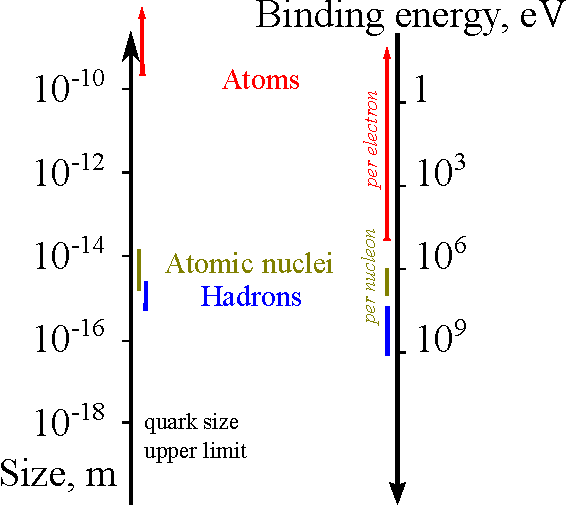
\includegraphics[height = 8cm]{illustrations/intro_illustrations/scales.pdf}
  \caption{Size and energy scales from atoms to quarks. This thesis deals in the
           range of atomic nuclei and hadrons.}
  \label{fig:scales}
\end{figure}

Heavy ions are the atoms of heavy elements (from Fe to U) with some or even all
of the electrons stripped off. Descending from larger to smaller length scale,
the physics of energetic heavy ion collisions involves atoms,
atomic nuclei, hadrons, quarks and gluons. The relevant spatial scales range
from the atomic scale of order $10^{-10}$ m down to
$10^{-16}$ m as shown in the left part of Figure \ref{fig:scales}. The
binding energy scales are demonstrated in the right part of Fig.
\ref{fig:scales} and range from eV to GeV per bound object.

The existence of atoms is of common knowledge nowadays, so atoms seem to be a
good starting point to discuss physics on smaller scales. Disassembling any
macroscopic object to smaller and smaller parts one will inevitably
arrive at atoms of one of the elements from the Mendeleev's periodic table:
hydrogen, carbon, oxygen, nitrogen, sulfur, iron, or any other of more than
110 elements. First introduced by ancient Greek philosophers Democritus and
Leucippus as purely theoretical objects, today atoms can be directly observed
in the electron microscope, moreover even manipulations with individual atoms
are possible.

Starting from Rutherford experiments (Nobel prize in chemistry 1908) it is
known that atoms have a dense nucleus, which is 1000 times smaller than the
whole atom, but contains 99.9 \% of its mass. The nucleus of size $1 -
10$ fm consists of nucleons (electrically charged protons and neutral
neutrons) bound together with energies from 1 to 8 MeV per nucleon.
Even the electrons in the inner shells of heavy elements are bound by at most
0.1 MeV per electron, so electrons can be detached from a nucleus
without destroying the nucleus itself. Initial ionization is experimentally
achieved by using strong electric fields, further ionization - by accelerating
the ions and letting them fly through thin stripping foils.

Protons, neutrons and electrons exist as well as individual particles.
Protons and electrons are stable outside of atoms (their measured average lifetime
upper bounds are larger than the age of the Universe).  Neutrons live around
880 s in average, decaying into a proton, electron and anti-neutrino. The
fact that all kinds of atoms consist of only 3 particles -
protons, neutrons and electrons - is indeed very satisfying, but it has turned
out that the whole particle zoo is much richer. Hundreds of short-living
particles were discovered during the past century in cosmic rays and in
high-energy proton-proton, proton-electron, electron-positron and other
collisions in particle accelerator experiments. The variety of discovered
particles has posed the question, which of them are fundamental and how they
can be classified.

\subsection{Elementary particles}

\begin{figure}
  \centering
  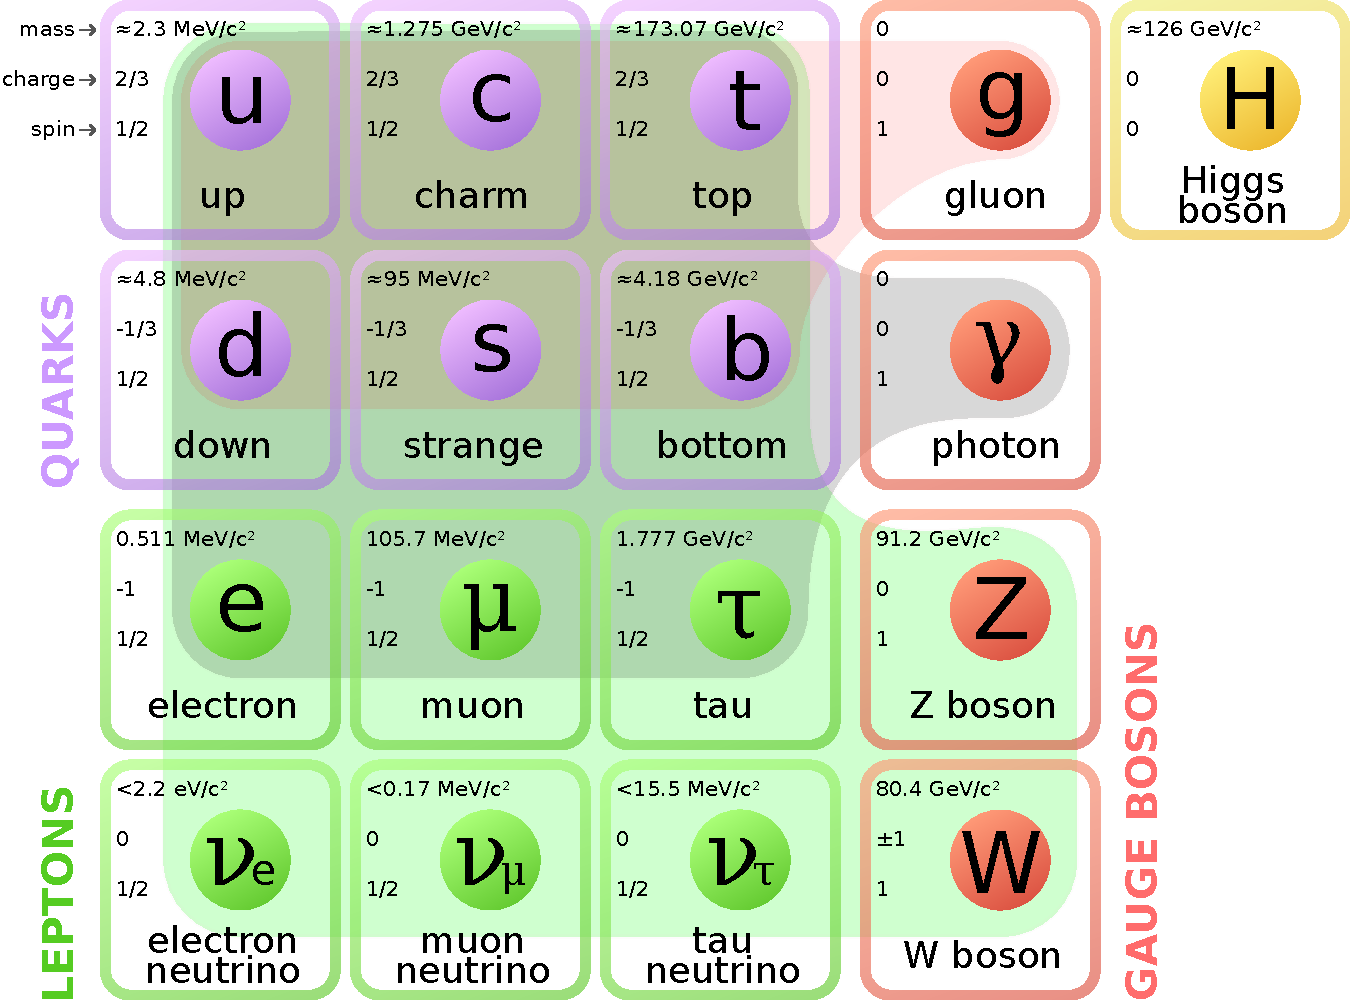
\includegraphics[width = 0.8\textwidth]{illustrations/intro_illustrations/Standard_Model.pdf}
  \caption{Elementary particles of the Standard Model, their properties and
           interactions \cite{elementary_particles_wiki}.}
  \label{fig:standard_model}
\end{figure}

Presently the above mentioned classification questions are answered by the
Standard Model of particles and interactions \cite{standard_model}.  Few
particles are considered to be elementary - by definition this means they are
point-like and do not have excited states.  Elementary particles can still be
unstable and decay into other elementary particles.  They are
characterized by mass, electric charge and spin - an intrinsic form of angular
momentum measured in units of $\hbar$. In Figure \ref{fig:standard_model} all
elementary particles are listed together with their properties according
to our present knowledge.

Depending on the spin, particles are classified into fermions (spin $\frac{1}{2}$,
$\frac{3}{2}$, $\frac{5}{2}$, etc) and bosons (spin $0$, $1$, $2$, etc). 
The difference between bosons and fermions is however not limited just to numerical
values of spin. It has a very deep
implication, manifested as the spin-statistics theorem: two fermions are not
allowed to be in the same quantum state (this rule is also referred to as Pauli
exclusion principle), while any number of bosons can be in the same quantum
state. It is due to Pauli's principle that electrons in atoms cannot reside on one
orbital, but create structures of orbitals that give elements their chemical
properties.  It also plays a role in atomic nuclei, because protons and
neutrons are fermions.  So are the quarks, of which they are composed of.

 In the Standard Model there are 12 fermions, 4 bosons with spin $1$ and the Higgs
boson with spin $0$.  All the interactions between fermions are described as an
exchange with a boson, that is why the bosons of the Standard Model are also called
force carriers. The exchange of a gluon $g$ corresponds to the strong interaction,
the exchange of $W^{\pm}$ or $Z$ bosons is the weak interaction and exchange of a
photon $\gamma$ describes the electromagnetic interaction. The Higgs boson was
introduced as a mathematical construction necessary to provide the $W^{\pm}$ and $Z$
bosons mass, which could not be introduced directly without violating gauge
symmetry.  In 2012 the Higgs boson was discovered as a physical particle. In 2013 a
Nobel prize was awarded to Englert and Higgs, who predicted the Higgs boson in 1964.


All 12 fermions in Fig. \ref{fig:standard_model} can interact weakly, i.e.
exchange $W^{\pm}$ or $Z$ bosons. However, only 6 of them interact
strongly, i.e. exchange gluons.  The strongly-interacting fermions are
called \emph{quarks}, the rest are called \emph{leptons}. Leptons include
electron, muon, tau-lepton and neutrinos. For every fermion there is also an
antiparticle, which has identical mass and spin, but opposite electric charge.
The first 3 columns of the table in Fig.  \ref{fig:standard_model} are called
generations. One can notice that  particles in each generation are
heavier than in the previous. This remains an observed fact and has no
underlying theoretical explanation.  Lighter three quarks, $u$, $d$ and $s$,
are often referred to as ''light quarks'', the rest are ''heavy quarks''. The
type of quark, one of the six possible, is also called flavour.

This thesis is devoted almost exclusively to the quark sector and the strong
interaction. The weak and electromagnetic interactions can be
neglected for the purposes of this thesis, because on the time scales of order
100 fm/c $\simeq$ $10^{-22}$ s, which are relevant for heavy ion
collisions, strong interactions are much more intense than all the
other interactions.
For example, it takes around $10^{-24}$ s to form a
pion in a proton-proton collision via strong interaction, $10^{-17}$ s
for it to decay  via electromagnetic interaction and $10^{-8}$ s to
decay via weak interaction. On the one hand, this allows to simulate heavy ion
collisions neglecting electromagnetic and weak interactions. On the other hand,
it makes photons and dileptons useful penetrating probes, which are emitted once and do not rescatter during the hadronic fireball evolution.


\subsection{Hadrons and color confinement} \label{sec:confinement}

So far, quarks and gluons were introduced as elementary particles subjected to the
strong interaction. In the following their property called ''color'' is introduced
and their bound states are discussed.

In general any particles may form bound states, if their interaction is
attractive.  For example \Pelectron and \Ppositron can form positronium,
\Pelectron and $\mu^+$ also form a bound state, connected by the electromagnetic
interaction. There are no known bound states produced purely by weak
interaction, although conjectured heavy neutrinos from extensions of the
Standard Model would form a bound state \cite{Dmitriev:2012ha}.
In contrast, strong interaction forms a plethora of bound states, called
\emph{hadrons}.

Not every combination of quarks and antiquarks appears as a bound state in
nature. Experimentally known are only $q\bar{q}$ states called \emph{mesons} and $qqq$
states called \emph{baryons}. Explaining the absence of states like $qq$ or $qq\bar{q}$
involves a property of quark called ''color''. It is unrelated
to the spectrum of reflected or transmitted light called color in our daily
life, but there is an analogy that will be explained further. Quark color has 3
eigenvalues, often denoted as $r$, $g$ and $b$. The number of colors $N_c = 3$
and the necessity to introduce it is justified by several reasons:

\begin{itemize}
\item Experimentally known hadrons like $\Delta^{++}(uuu)$ or $\Omega^-(sss)$
      would be forbidden by the Pauli principle, if the only quantum number of
      quarks was the spin. The measured spin of $\Delta^{++}$ is $3/2$, which implies
      that every $u$ quark that it is composed of has spin projection $1/2$. So
      without additional quantum numbers all $u$-quarks are in the same quantum
      state, which violates Pauli principle. With color $\Delta^{++}$ and $\Omega^-$
      are allowed by Pauli principle, because every quark is in a different color
      state.
\item A number of experiments have measured the ratio of produced hadrons
      to $\mu^-\mu^+$ pairs in \Pelectron\Ppositron collisions,
      $R = \frac{\sigma(e^+e^- \to \mathrm{hadrons})}{\sigma(e^+e^- \to \mu^+\mu^-)}$.
      This ratio is proportional to $N_c$ and measurements indicate $N_c = 3$.
\item If one takes the standard model with an arbitrary number of colors $N_c$,
      then it would be non-renormalizable because of the so-called axial anomaly in
      the electroweak sector. The anomaly is only canceled for $N_c = 3$. As a side
      note, this anomaly cancellation also requires that fermions are grouped into
      quark-lepton families.
\item All the hadrons found in nature are invariant under
      transformations in the color space, or in mathematical terms,
      hadrons are singlet representations of the $\SUgroup{3}$ group (more details are
      given in the appendix \ref{sec:SU3}). Here the
      analogy with our daily life color comes into play: like red, green and blue
      superimposed result in white, colored quarks compose ''colorless'' hadrons. Here
      ''colorless'' actually means that hadrons do not change - are invariant - under
      the $\SUgroup{3}$ transformations in color space. It turns out (see appendix
      \ref{sec:SU3} for details) that combinations $qqq$, $q\bar{q}$,
      $q\bar{q}q\bar{q}$, $qqqq\bar{q}$ have singlet representations of $\SUgroup{3}$
      group and thus can be colorless, while combinations like $qq\bar{q}$, $qq$,
      $qqqq$ or single quarks cannot be colorless by any means.
\end{itemize}

The observed existence of only colorless objects in nature is often referred to as
\emph{color confinement} or simply confinement, because the color is confined inside
of hadrons.  To acknowledge the role of color, the microscopic quantum field theory
describing the strong interaction is called quantum chromodynamics (see section
\ref{sec:QCD} for details). In addition to baryons and
mesons color confinement allows many other combinations of quarks, including the
pentaquark $qqqq\bar{q}$. Remarkably, in 2015 two kinds of pentaquarks were
discovered by the LHCb collaboration at the Large Hadron Collider at CERN
\cite{Aaij:2015tga}.

% PDG: www-pdg.lbl.gov/2015/listings/rpp2015-list-free-quark-searches.pdf
Confinement implies that no single free quark can be observed. This statement
has been tested experimentally by multiple experiments \cite{Agashe:2014kda},
measuring the cross-section for the inclusive reaction

\begin{equation}
  pp \to q(\bar{q}) X \,. \nonumber
\end{equation}

The best upper limit for the cross-section of such a reaction is currently set by the
CMS collaboration and constitutes $\sigma < $ $2.3 \times 10^{-40}$ cm$^2$.
This has to be compared to the total $pp$ cross-section, which is of order
100 mb or $10^{-25}$ cm$^2$. This implies that if single quarks
are produced in $pp$ collisions then at the maximum average rate of $10^{-15}$ per
collision. So far no single quark was observed.

Quantum chromodynamics (QCD) explains confinement in the following way.
From the lattice formulation of QCD one can obtain a phenomenological
quark-antiquark potential

\begin{equation}
  V(r) = -\frac{\alpha}{r} + \kappa r \,,
\end{equation}

which grows with distance. If one tries to separate a quark and an antiquark and
pull them apart, their interaction energy is large enough to produce a new
quark-antiquark pair out of vacuum. So, instead of a separated quark and antiquark
one obtains two mesons. This explanation does not provide a full understanding
of confinement. For example, it is still unclear under which conditions quarks
are not confined.

QCD predicts that at high collision energy the interaction between quarks becomes
small. This phenomenon is called asymptotic freedom (see section \ref{sec:QCD}). The
asymptotic freedom implies that there is a possibility to obtain deconfined quarks
at sufficiently high temperature and density.

\subsection{Quark-gluon plasma}

\begin{figure}
  \centering
  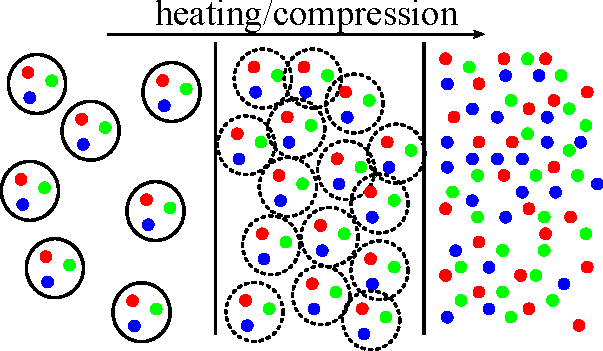
\includegraphics[width = 0.6\textwidth]{illustrations/intro_illustrations/qgp.pdf}
  \caption{Hadrons with confined color turn into a gas of quarks
           with deconfined color at heating and/or compression.}
  \label{fig:qgp}
\end{figure}

As mentioned before, it follows from asymptotic freedom of QCD that very hot
and/or very dense matter consists of almost non-interacting quarks. It
was suggested \cite{Collins:1974ky} that by heating and compressing matter in
high-energy heavy ion collisions one obtains an almost ideal gas of
\emph{deconfined} quarks. The naive illustrative picture of this is shown in
Figure \ref{fig:qgp}.

Asymptotic freedom was established theoretically in the framework of 
zero-temperature field theory for the interaction of two quarks. In a heavy ion
collision the physics is significantly different: the size of the system is much
larger than the size of a single nucleon and one can therefore speak of the formation
of a medium. Will the asymptotic freedom hold in the thermal bath created
by the medium? This question was answered by Eduard Shuryak in 1978 in the
one-loop approximation. He computed the gluon propagator and the potential
between two quarks in the thermal medium of temperature $T$ \cite{Shuryak:1977ut}:

\begin{align}
  V(r) = \frac{Q}{4 \pi r} \eexp{-m r} \\
  m^2 = \frac{1}{3} g^2 (N_c + N_f/2) T^2
\end{align}

This potential is similar to the Debye screening potential in a classical plasma,
therefore the hot and dense medium of quarks was called quark-gluon plasma.  It has
been produced experimentally at the Relativistic Heavy Ion Collider (RHIC) in 2000
\cite{Adams:2005dq,Adcox:2004mh,Arsene:2004fa,Back:2004je}.
Additionally it has been shown that the quark-gluon plasma behaves like a fluid with a
very low viscosity \cite{Song:2007ux,Dusling:2007gi,Romatschke:2007mq}. Low viscosity
implies that the QGP obtained in Au+Au collisions at RHIC is strongly-coupled, in
contrast to an earlier picture of a weakly-couple gas (see \cite{Shuryak:2008eq} for
a review of this paradigm shift).

What are the physical properties of the quark-gluon plasma? How and under which
conditions does the transition from hadronic matter to the quark-gluon plasma occur?
Is there a phase transition or only a smooth cross-over? If phase transition then of
which order? Is there a critical point and if yes, where is it located and what are
the critical indices? Are there additional phases? These are some of the
questions that motivate modern heavy ion collision experiments and theoretical
investigations. Many of these questions are directly related to the phase
diagram of the strongly-interacting matter.

\subsection{Phase diagram of strongly-interacting matter}

\begin{figure}
  \centering
  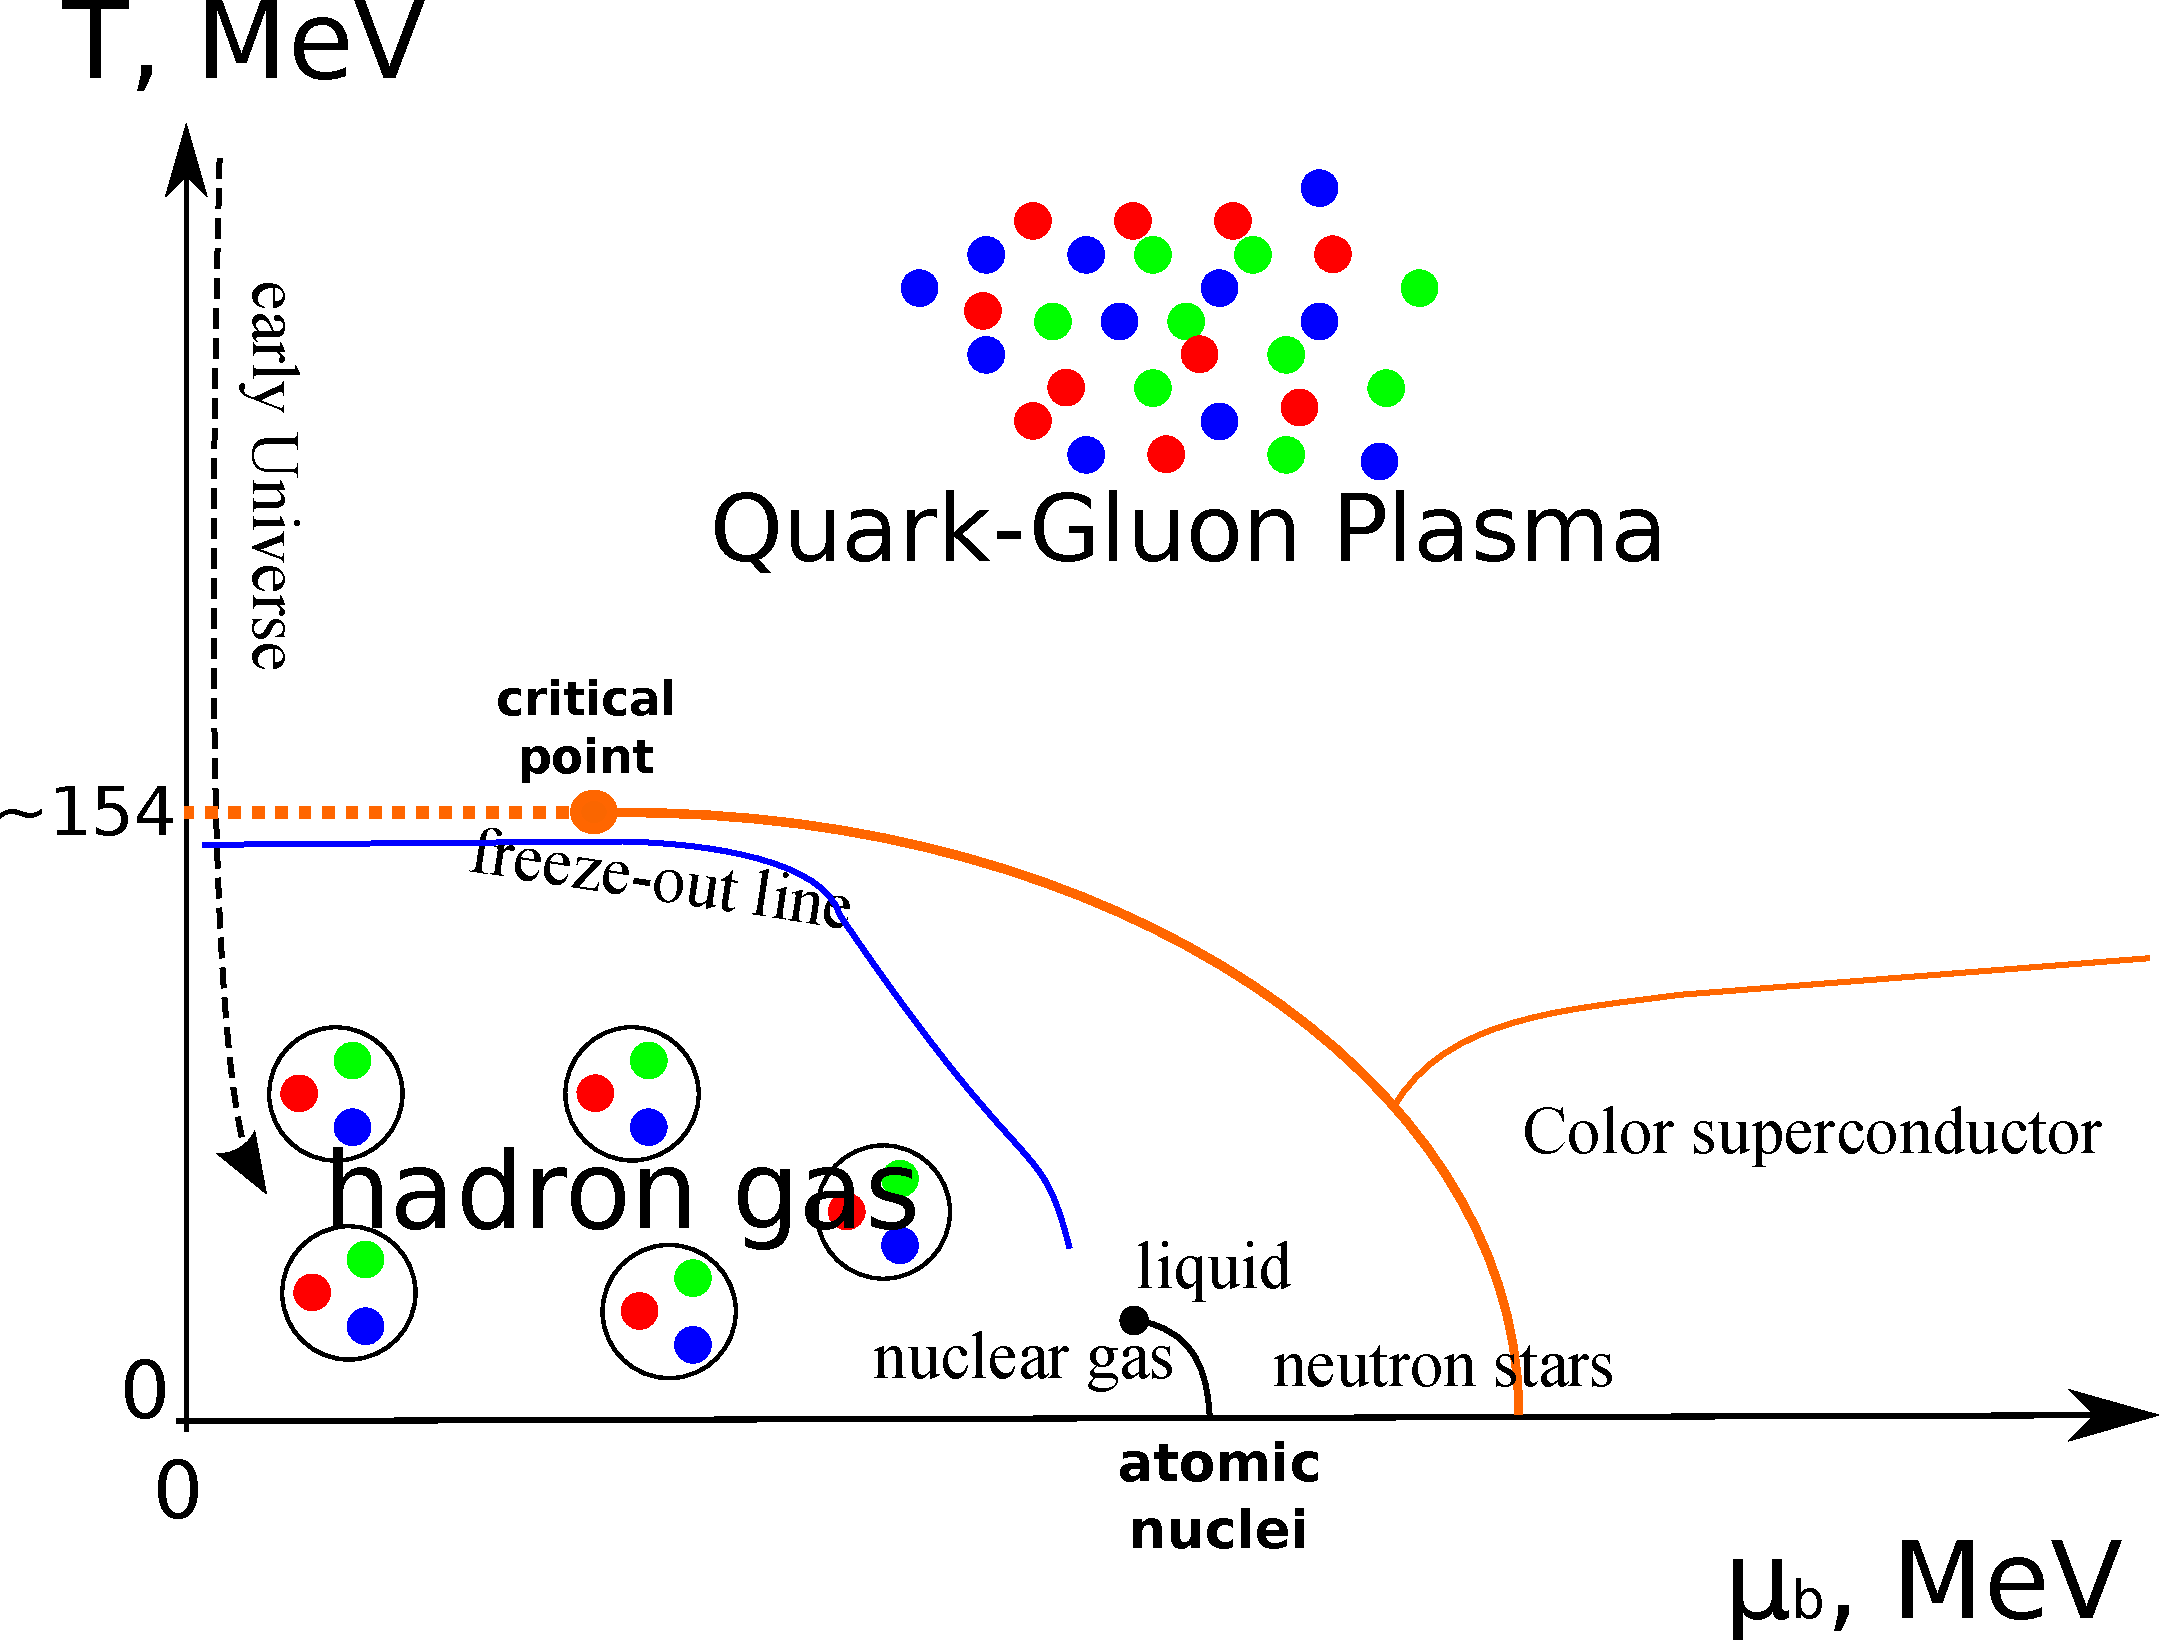
\includegraphics[width = 0.7\textwidth]{illustrations/intro_illustrations/phase_diagram.pdf}
  \caption{Schematic phase diagram of strongly-interacting matter.}
  \label{fig:phase_diagram}
\end{figure}

One of the most important tasks of modern heavy-ion collision experiments is
to study the phase diagram of strongly-interacting matter
\cite{BraunMunzinger:2008tz}. A sketch of the theoretical and experimental
knowledge about the phase diagram is given in Figure \ref{fig:phase_diagram} in
terms of temperature $T$ and baryon chemical potential $\mu_b$. The chemical potential
refers to the energy increase of the system after adding one baryon, it also
characterizes the asymmetry between baryons and antibaryons. At $\mu_b = 0$ the
energies needed to add a baryon or an antibaryon to the system are identical and
therefore baryon and antibaryon numbers are equal. At high $\mu_b$ baryons are
strongly preferred.

Strictly speaking, the diagram can have two additional axes, isospin chemical
potential $\mu_{I3}$ and strangeness chemical potential $\mu_s$. On this
diagram, it is assumed that $\mu_s=\mu_{I3} = 0$.  Non-zero isospin chemical
potential is important for neutron stars, because it characterizes the asymmetry
between protons and neutrons, which is significant in these cosmological systems.
More important for heavy ion collisions is the transition between hadron gas
and quark-gluon plasma. At high collision energies approximately equal amounts
of baryons and antibaryons are produced, so $\mu_b$ is small. The region of
$\frac{\mu_b}{T} \le 2$ is covered by lattice QCD calculations
\cite{Borsanyi:2013bia,Bazavov:2014pvz,Bazavov:2017dus}, which conclude that in
this region there is no phase transition, only a smooth cross-over.  The value
of the pseudocritical temperature where the chiral susceptibility has its maximum
is $T_c = $ 153 MeV \cite{Aoki:2006br,Borsanyi:2010bp,Bazavov:2011nk}.
Unfortunately, lattice QCD is limited to the vicinity of $\mu_b = 0$ due to
the sign problem \cite{deForcrand:2010ys}.


At non-zero $\mu_b$ a first-order phase transition is predicted by multiple
models and phenomenological studies (see summaries in \cite{Stephanov:2004wx}
and~\cite{Lacey:2014wqa}). A first order phase transition occurs in massless
two-flavour QCD \cite{Berges:1998rc,Halasz:1998qr} as well as in the two flavour
linear sigma model and Nambu-Jona-Lasinio model~\cite{Scavenius:2000qd}, in a
model based on the statistical bootstrap~\cite{Antoniou:2002xq} and in a model
with an effective potential for two-flavour massive QCD~\cite{Hatta:2002sj}.
However, none of these models can be described as fully realistic.
%Alba_realistic->complete? 
The point where the first order phase transition ends and cross-over starts is
called critical point. In the vicinity of the critical point multiplicity
fluctuations become large \cite{Stephanov:2008qz,Stephanov:1999zu}. At RHIC
and at NA61 experimental measurements of multiplicity fluctuations are ongoing
to locate the critical point. Future FAIR, NICA and J-PARC facilities have
search and possibly studies of the critical point as a part of their motivation
(see more in section \ref{sec:HI_exp}).


The nuclear matter liquid-gas phase transition with its own critical point
around $T_c^{\mathrm{nucl}} \approx $ 20 MeV was studied both
theoretically and experimentally in ion collisions
\cite{Panagiotou:1984rb,DAgostino:2005qpq}. There are many indications in
favor of a phase transition. These include temperature saturation over a broad
range of energies, flattening of the caloric curves, sudden opening of the high
fragment multiplicity channel, the onset of collective expansion, the
abnormally high partial energy fluctuations, the bimodal distribution of
exclusive observables, and the finite size and Fisher scalings. However, the
numerical value of the critical point still has a large uncertainty and even the
discovery of the transition is still debatable.

The color superconductor phase was theoretically predicted at very large baryon
densities and low temperatures \cite{Alford:1998mk,Schafer:1999fe}. At these
high densities, possibly occurring in the cores of neutron stars, gluons acquire
large mass, as quarks form a condensate and massive excitations over condensate
dominate physics, so that ''QCD at high densities and low temperatures may in
many ways be much more similar to QCD at low densities than to a weakly coupled
quark-gluon plasma'' \cite{Rajagopal:1998ec}.

The chemical freeze-out line results from an attempt to quantify features of the
phase diagram from the experimental side \cite{Andronic:2005yp}. By definition
chemical freeze-out is the instant, when inelastic number-changing hadronic
reactions cease, because of the expansion of the system, and hadron multiplicities
are fixed, ''frozen''. The thermal (also called ``hadron resonance gas'') model
postulates simultaneous sharp chemical freeze-out for all hadron species. Despite
this rough approximation, this model provides a surprisingly
good description of hadron multiplicities in heavy ion collision for collision
energies ranging from a few GeV per nucleon pair to 2.76 TeV
\cite{Cleymans:1999st,Andronic:2005yp,Stachel:2013zma}.  Temperature $T^{FO}$
and chemical potential $\mu_b^{FO}$ at the chemical freeze-out are parameters of
thermal models extracted from fitting multiplicities at each
experimental collision energy. Lattice QCD studies hint that the freeze-out curve
lies near the phase transition curve for low $\mu_b$ \cite{Kaczmarek:2011zz}.

Different parts of the phase diagram are studied with different theoretical
approaches and it is an important task to connect them. Describing different parts of
the phase diagram in a unified approach would allow
to connect properties of neutron stars, heavy ion collision experiments at
high energies and measurements of the nuclear phase transition.

\subsection{Big bang and neutron stars}

The physics of hadrons and quark-gluon plasma has deep connections to cosmology, in
particular to the early universe evolution and to neutron stars. Our universe is
known to be uniform on a very large scale of 100 Mpc, but it is extremely
non-uniform on a smaller scale. Indeed, the density of neutron star is 40
orders of magnitude larger than the density of cosmic voids. It is suggested that
the phase transition from a hot quark-gluon plasma to hadrons during the first
microseconds after the Big Bang could be partly responsible for such a non-uniformity.
For example, in \cite{Witten:1984rs} lumps of quark matter floating in
the Universe are suggested and in \cite{Kapusta:2000fe} the impact of the QCD
transition on inhomogeneities in the baryon to photon ratio is studied.

After the Big Bang the universe was extremely hot, small and was cooling and
expanding \cite{Weinberg:1977ji}, similarly to the fireball in heavy ion
collisions, although the initial temperature was higher - of order
$10^{18}$ GeV at Plank time of $10^{-43}$ s in contrast to
initial temperatures of several hundred MeV in heavy ion collisions.
At $10^{-7}$ s the Universe has already reached conditions testable in
modern heavy ion collisions experiments.  Of course, between the universe and
ion collisions there are differences in geometry. The expansion of the universe
was spherical, while heavy ion collisions have a collision axis. However, due to
the formation of a quark-gluon plasma, similarities in expansion and cooling and
also in the sequence of freeze-out processes heavy ion collisions are sometimes
called the Little Bang.

Hadronic and quark-gluon plasma physics are also related to neutron stars and
conjectured quark stars \cite{Xu:2002wd}. Neutron stars are remnants of type II
supernovae explosion, typically detected as millisecond radio pulsars. They can
neither be too light, otherwise they would be destroyed by centrifugal force;
nor too heavy to avoid collapse into a black hole. Observed neutron stars have
masses approximately between 1 and 2 solar masses and radius from 10 to 20
kilometers \cite{Lattimer:2012nd}. Simultaneous precise measurements of mass,
radius and rotation period of neutron stars would put stringent constraints on
the nuclear equation of state at high densities. For example, precise
measurements of the masses of PSR J1614-2230 ($M =  1.97 \pm 0.04 M_{Sun}$)
and PSR J0348-0432 ($M = 2.01 \pm 0.04 M_{Sun}$)
\cite{Demorest:2010bx,Antoniadis:2013pzd} have excluded many quark matter
equations of state, which could not produce such heavy neutron stars.
Nevertheless, there is still enough room for stars with quark core
\cite{Alford:2013aca,Benic:2014jia}.  Astrophysical measurements of neutron
stars probe the lower temperature and high density region of the phase diagram
in Fig. \ref{fig:phase_diagram} and are thus complementary to heavy ion
collision studies.

\subsection{Structure of the thesis}

Going from atoms to neutron stars, the introductory part of this thesis has outlined
the general motivation driving heavy ion collision experiments and theoretical
calculations all over the world. Section \ref{sec:HI_exp} overviews the
experimental studies of heavy ion collisions and demonstrates substantial
interest on intermediate energies, where the search of the critical point is or
will be performed. Section \ref{sec:HI_th} constitutes a brief overview of theory
related to heavy ion collisions. This is necessary to show the inter-relations
between different theoretical approaches and to introduce transport, hydrodynamical
and hybrid approaches, which play a big role in this thesis.

Chapter \ref{ch:interfaces} contains a mathematical part of methodology necessary
for the next parts. It provides a detailed description of the coarse-graining method,
fluidization and particlization - the interfaces between hydrodynamics and transport,
studied in this work.

The assumptions behind hydrodynamical and hybrid approaches that were fulfilled
at high energies may become challenging at intermediate energies. The first of these
assumptions is rapid thermalization over the whole fireball volume in heavy ion
collisions. The local thermalization at energies $\Elab = 5-160$ GeV per nucleon
($\sqrt{s_{NN}} = $ 3-17 GeV) is studied in a coarse-grained transport
approach in chapter \ref{chap:local_equilibration}.  The degree of
thermalization is estimated by quantifying local deviations of energy-momentum
tensor and baryon four-current in the Landau rest frame from the thermal equilibrium.
chapter \ref{chap:local_equilibration} is based on publication \cite{Oliinychenko:2015lva}.

Another assumption adopted by hydrodynamical and hybrid approaches at high
energies is that particles emitted from the region of hydrodynamical evolution
cannot return back and cause feedback to hydrodynamics. Neglection of
this feedback is typically manifested as so-called ''negative Cooper-Frye
contributions'' - negative numbers of particles emitted from certain regions of
the phase-space. At high energies at midrapidity they are negligible. Does this
hold for intermediate energies?  This question is investigated in chapter
\ref{chap:cooper_frye} based on publication \cite{Oliinychenko:2014tqa}.

Chapter \ref{chap:smash} (based on \cite{Weil:2016zrk}) introduces the SMASH
transport approach, which was used for the following computations.
In chapter \ref{chap:forced_therm} (based on \cite{Oliinychenko:2016vkg})
a novel approach to simulate hydrodynamical regime at high density
avoiding negative Cooper-Frye contributions is suggested and tested.
This approach is based on performing forced canonical thermalization in the
high-density region of the pure hadronic transport.
Chapter \ref{chap:summary} summarizes the main results of this work.

\section{Heavy-ion collision experiments} \label{sec:HI_exp}

%\begin{sidewaysfigure} \centering \includegraphics[width =
%\textwidth]{illustrations/intro_illustrations/mindmap/Heavy_ion_collisionsexperiments.pdf}
%\caption{Heavy ion collision experiments of the past (grey), present (red) and
%future (blue) with beam kinetic energy $\Elab > $ 1 GeV.}
%\label{fig:HIC_exp_mindmap}
%\end{sidewaysfigure}

\begin{table}
 \footnotesize
 \caption{Summary of heavy ion accelerators at energy $\Elab > $ 1 GeV.
          Operation time is given only for heavy ion period: e.g. Bevalac started
          operation in 1960, but heavy ion program was initiated in 1971.
          Note that only accelerated projectile ions are listed in the table, but not target
          ions.}
 \label{tab:HI_accelerators}
\begin{tabular}{llllllm{1cm}m{2cm}l}
  \toprule
  Accelerator                       &  Place                         &  Lab.  & Time       & $E_{beam}$ [GeV]    & $\sqrt{s_{NN}}$ [GeV]   & Projectile ions           & HI Experiments  & Refs.\\
  \midrule
  Bevalac                           & \pbox{20cm}{Berkley\\USA}       & BNL          & 1971-1993  & 0.4 - 2.1           & 2 - 2.7                 & O, C, Ne, Fe, Xe, U  & Plastic Ball, Streamer chamber, EOS, DLS & \cite{Barale:1975bb,Alonso:1982md} \\
  \midrule
  \pbox{20cm}{Synchro-\\Phasotron}  & \pbox{20cm}{Dubna\\Russia}      & JINR         & 1970-2003  & 0.1 - 4.5           & 1.9 - 3.5               & d - Si       &  & \cite{Malakhov:2013zjq} \\
  Nuclotron                         &                                 &              & 1993-now   & 0.1 - 4.5           & 1.9 - 3.5               & d - Xe, Au   & BM@N & \cite{Kovalenko:2016qmy,Kuznetsov:2016ynd} \\
  NICA                              &                                 &              & 2023-      & 2 - 5.5             & 4 - 11                  & d - Au       & MPD &  \cite{Kozlov:2016nbo, Kekelidze:2012zz} \\
  \midrule
  SIS18                             & \pbox{20cm}{Darmstadt\\Germany} & GSI          & 1990-now   & 0.1 - 2             & 1.9 - 2.7               & d - Au, $\pi$ & FOPI, HADES, KaoS & \cite{cbm_physics_book} \\
  SIS100(300)                       &                                 &              & 2022-      & $<$ 14 (44)         & $<$ 5.5 (9.2)           & d - U, $\pi$ & CBM, PANDA, NUSTAR & \cite{cbm_physics_book} \\
  \midrule
  AGS                               & \pbox{20cm}{Brookhaven\\USA}    & BNL          & 1980-1999  & 2 - 14.5            & 2.7 - 5.5               & O, Si, Au    & E802, E859, E866, E917, E814, E877, E810, E891, E895, E910 & \cite{cbm_physics_book, AGS_exp} \\
  RHIC                              &                                 &              & 2000-now   & 3.85 - 100          & 7.7 - 200               & Au, Cu, U, d & STAR, PHENIX, PHOBOS, BRAHMS   & \cite{RHIC_lumi} \\
  \midrule
  SPS                               & \pbox{20cm}{Geneva\\Switzerland}& CERN         & 1983-now   & 20 - 200            & 6.3 - 19.4              & O, S, In, Pb & NA35, CERES(NA45), NA49, NA57, NA60, WA98, NA61 (SHINE) & \cite{cbm_physics_book,Pugh:1989eb} \\
  LHC                               &                                 &              & 2008-now   & 1380 (Pb)           & \pbox{20cm}{2760 (PbPb)\\5400 (pPb)} & Pb & ALICE, ATLAS, CMS, LHCb & \cite{Armesto:2015ioy} \\
  \midrule
  MR                                & \pbox{20cm}{Tsukuba\\Japan}     & JPARC        & 2024-      & 1 - 19              & 2 - 6.2                 & d - U        &   & \cite{Sako:2015cqa} \\
 \bottomrule
\end{tabular}
\end{table}

An important part of the motivation for this thesis stems from ongoing and
planned heavy ion experimental programs. That is why in this section a short overview
of heavy ion experiments is given. Only experiments with the relativistic beam of
kinetic energy $\Elab > $ 1 GeV per nucleon are considered. This
condition cuts off heavy ion programs devoted to nuclear physics, such as heavy
ion experiments in Saclay (France), Uppsala (Sweden), East Lansing (USA) or
RIKEN experiment (Japan). In the world there is only a limited number of
accelerators operating at $\Elab > $ 1 GeV per nucleon, the information
about them is summarized in table \ref{tab:HI_accelerators}. They are all
synchrotrons with a beam revolving continuously in a circular beam pipe.
Typically multiple experiments are taking advantage of the beam.

% Lowest energy: Bevalac, Synchrophasotron, SIS18
Pioneering experiments in heavy ion collisions were performed in the 1970ies at
Bevalac at Lawrence Berkley Laboratory (LBL) in the US and at Synchrophasotron in
Dubna (Russia). They managed to create compressed nuclear matter and study
its properties. The most important results of Bevalac include studies of the
equation of state of nuclear matter \cite{Brown:1990pp}, collective phenomena
\cite{Doss:1986eh,Gustafsson:1984ka} and low-mass dileptons
\cite{Roche:1988er}.  Synchrophasotron studied cumulative effect,
HBT-correlations\cite{Lisa:2005dd} and nuclear multifragmentation
\cite{Kuznetsov:1982zc}.  These
experiments were operating at beam energies below 2 GeV per
nucleon. In 1990 SIS18 started to operate in the same energy regime. SIS18
experiments FOPI and KaoS have performed systematic studies of pion production
\cite{Reisdorf:2006ie}, strangeness production
\cite{Laue:1999yv,Wisniewski:2001dk} (including subthreshold production of
$\Sigma$-baryon \cite{Lopez:2007zz} and $\phi$-meson \cite{Mangiarotti:2002mw})
and collective flow studies \cite{Andronic:2000cx}.  HADES continues these
studies \cite{Stroth:2017blf} and extends them to investigations of dilepton
production \cite{Agakishiev:2011vf,Franco:2017ano}. Hadronic transport approaches were
successfully applied to describe the results of experiments at Bevalac and
SIS18.

% Low energy: AGS
Beam energies of $\Elab$ = 2 - 14.5 GeV ($\sqrt{s_{NN}} = $ 2.7 -
5.5 GeV) were covered by the Alternating Gradient Synchrotron (AGS) at
Brookhaven National Laboratory, first colliding lighter $^{16}$O and $^{28}$Si
nuclei and then heavier $^{197}$Au nuclei.  Exclusive particle spectra
\cite{Ahle:2000wq,Ahle:1999va,Ogilvie:1997mb} were measured for $\pi^{\pm}$,
$K^{\pm}$, $p$, $\bar{p}$, $\Lambda$, $\bar{\Lambda}$ and $\varphi$. Directed
($v_1$) \cite{Barrette:1995cv} and  elliptic ($v_2$) flow
\cite{Barrette:1996rs} were investigated.  Pion interferometry
\cite{Lisa:2000xj} allowed to extract the produced fireball size. The overall
conclusion was that ``there is no evidence for any onset of new behavior beyond
hadronic scattering as the beam energy or centrality is
changed''~\cite{Kahana:1997aq}, because the results of AGS were well-reproduced
by the hadronic transport models RQMD and ARC \cite{Kahana:1997aq}. Another
conclusion was that the produced particle multiplicities correspond to thermal
equilibrium in the grand-canonical ensemble \cite{BraunMunzinger:1994xr}, which
turns out to be true also for higher collision energies.

% Intermediate energy: SPS
At the Super Proton Synchrotron (SPS) at CERN a sequence of experiments
was carried out using oxygen, sulfur and lead
beams at $\Elab = $ 20-200 GeV per nucleon corresponding to
$\sqrt{s_{NN}} = $ 6.4-19.4 GeV. At the highest SPS energy NA35
experiment reached the theoretically required energy density for
quark-gluon plasma formation in S+S collisions~\cite{Pugh:1989eb}. The goal of
the later experiments in a larger Pb+Pb system was to look for the onset of
quark-gluon plasma formation by decreasing collision energy. The experiments NA45,
NA50 and WA98 measured low-mass dielectron spectra \cite{Wessels:2002ha},
dimuon spectra \cite{Ramello:2003ig} and direct photons \cite{Aggarwal:1998vs}.
NA57 has measured multistrange hadron production \cite{Bruno:2004pv}. Very
extensive and systematic measurements of hadron production were conducted by
NA49 experiment \cite{Bachler:1999hu}.  Overall, big attention at SPS was
devoted to electromagnetic and strange particle observables as potential
signals of the quark-gluon plasma formation.  Among these signals are ''Kink,
Step and Horn'' \cite{Gazdzicki:2010iv,Rustamov:2012np}: a sharp maximum in the
$\frac{K^+}{\pi^+}\parenths{\sqrt{s}}$ (Horn), sudden change in the number of
pions per participant (Kink) and a plateau in the $\sqrt{s}$ dependence of
inverse slop parameter of the kaon transverse momentum spectra (step). Hadronic
transport models were unable to describe the Horn and especially the Step
\cite{Bratkovskaya:2003ny}. This is consistent with the hypothesis of
quark-gluon plasma observation, although does not serve as unambiguous
evidence.  NA61, the successor of NA49 experiment, is now operating at the same
energies that NA49, but with a broader range of collision system sizes
\cite{Gazdzicki:2011fx}. NA61 also puts more attention to measuring hadron
multiplicity fluctuations.

%RHIC
The Relativistic Heavy Ion Collider (RHIC) at Brookhaven National Laboratory
started its operation in 2000 using AGS as a preaccelerator. The beam time at RHIC is
dedicated almost completely to heavy ion collisions (there is also a polarized
proton collision program). Unlike all the previous experiments, RHIC is a
collider. Initially experiments at a center of mass collision energy of
$\sqrt{s_{NN}} = $ 200 GeV and 130 GeV per nucleon were conducted. Later the
Beam Energy Scan program was launched with the motivation to find the critical
point of the phase diagram (see Fig. \ref{fig:phase_diagram}) and the collision
energy was systematically decreased down to 7.7 GeV at the cost of beam
luminosity \cite{RHIC_lumi}. The smallest experiment at RHIC, PHOBOS, has
measured global observables, including charged particle multiplicities, in a
large window of rapidity \cite{Alver:2010ck}.  BRAHMS, PHENIX and STAR have
performed systematic measurements of hadronic spectra
\cite{Chujo:2002bi,Kumar:2011us}, collective flow of identified hadrons
\cite{Agakishiev:2011eq,Lacey:2001va}, jet quenching, heavy flavour,
fluctuations and correlations in large Au+Au/Cu+Cu and in small d+Au
systems.  The spectra and elliptic flow of identified particles at low
transverse momentum is well-described by  ideal relativistic hydrodynamics
\cite{Kolb:2000fha,Huovinen:2001cy,Hirano:2002ds}, as well as by hydrodynamics
with hadronic afterburner \cite{Teaney:2001gc}.  This led to the statement that a
nearly ideal fluid was created at RHIC
\cite{Adams:2005dq,Adcox:2004mh,Arsene:2004fa,Back:2004je}. Viscous
relativistic hydrodynamics was applied to describe the RHIC $v_2(p_T)$ data
\cite{Song:2007ux,Dusling:2007gi,Romatschke:2007mq} and it was shown that an
extremely low viscosity to entropy density ratio $\frac{\eta}{s}$ from 0.08 to
0.2 \footnote{Dimensionless since $k_B = \hbar = c = 1$ is used, in SI has
dimension $\frac{k_B}{\hbar}$.} is preferred by data. The applicability of
hydrodynamics, early thermalization, high $v_2$ and low $\eta/s$ signal that
a strongly-interacting fluid is produced at RHIC.  Additional convincing
arguments that this fluid is indeed the quark-gluon plasma were jet quenching
\cite{Betz:2012hv}  and the scaling of $v_2$ with the number of constituent quarks
\cite{Xu:2005jt,Adamczyk:2013gv} (although constituent quark scaling being a
signature of quark-gluon plasma is debatable \cite{Lu:2006qn}).  Currently, the RHIC
beam energy scan is focused on the search of the critical point and therefore
event-by-event fluctuations of conserved charges became important observables
\cite{Adamczyk:2013dal}.

The Large Hadron Collider (LHC), which started its operation in 2010, has
contributed significantly to the field of heavy ion collisions. LHC makes use
of a specialized detector ALICE (A Large Ion Collider Experiment) dedicated to
heavy ion collisions, but also CMS (Compact Muon Solenoid), ATLAS (A Toroidal
LHC ApparatuS) and LHCb play significant role in heavy ion measurements.  LHC,
in addition to its main $p+p$ program, is colliding $Pb+Pb$ at $\sqrt{s_{NN}} =
$ 2.76 TeV, as well as $p+Pb$ at $\sqrt{s_{NN}} = $ 5 TeV.
With energy an order of magnitude higher than at RHIC, there is no doubt in the
literature that the quark-gluon plasma is produced at LHC. HBT correlation 
measurements (see \cite{Lisa:2005dd} for explanation of the method) show
that the hot and dense fireball at LHC is larger than at RHIC and leaves longer
until decoupling \cite{Aamodt:2011mr}. Fourier harmonics of $\frac{dN}{d\phi}$
were measured up to $v_6$ and are well-described by hydrodynamics. Jet
quenching turned out to be smaller than at RHIC consistently with perturbative
QCD predictions. The biggest surprise from LHC was that the smaller systems like
$p+Pb$ or high-multiplicity $p+p$ were exhibiting large $v_2$ and were
described well by hydrodynamics, which seems to be consistent with the production
of quark-gluon plasma.

Future experiments are dedicated to the search of the critical point of strongly
interacting matter and a possible phase transition between hadrons and
quark-gluon plasma. The future accelerators are FAIR (Facility for Antiproton and Ion
Research, includes SIS100 accelerators)~\cite{Spiller:2006gj} at GSI
(Gesellschaft f\"ur Schwerionenforschung) in Darmstadt, Germany; NICA
(Nuclotron-based Ion Collider fAcility)~\cite{Kekelidze:2012zz} at JINR in
Dubna, Russia; and JPARC-HI~\cite{Sako:2015cqa} at Japan Proton Accelerator
Research Complex (JPARC) in Japan. All of them concentrate on the intermediate
or lower energy region, where the critical point and the first-order phase
transition are expected.  NICA will be a collider using the existing Nuclotron as
an injector.  This will allow to increase energy to $\sqrt{s} = $
4-11 GeV, accelerating all kinds of ion beams. FAIR will be a major
addition to SIS18 accelerator at GSI, operating with fixed target at low
energies up to $\sqrt{s} = $ 4.9 GeV at a very high beam rate and with
possibility of antiproton and rare isotope beams. JPARC-HI energies are
$\sqrt{s} = $ 2-6.2 GeV and the high beam rate is planned, as for FAIR,
of order $10^{11}$ ions per cycle.

Two observations can be drawn from this brief heavy-ion experiment overview.
Firstly, the experimental interest is shifting towards lower and intermediate
energies.  This is manifested by the RHIC beam energy scan program, NA61 at
SPS, as well as future experiments FAIR, NICA and JPARC-HI.  Secondly, with
some exceptions the results of the low-energy experiments are well-described by
hadronic transport approaches and the results of high-energy experiments are
well-described by the hydrodynamics. Understanding the results of future
experiments at intermediate energies requires extending theoretical approaches
calibrated at low and high energies.

The terms ``low energy'', ``intermediate energy'' and ``high energy'' are frequently
used throughout the thesis. The ranges are defined only approximately and are
partly motivated by the experimental programs. Table \ref{tab:energies_convention}
summarizes the convention adopted in the text.

\begin{table}
  \begin{tabular}{lll}
   \toprule
    Collision energy     &   $\sqrt{s}$ [GeV]  &   Accelerators \\
   \midrule
     ``Low''             &   $\lesssim$ 4.5    & Bevalac, Nuclotron, SIS, AGS \\
     ``Intermediate''    &   $\approx$ 5 -- 20 & SPS, RHIC (BES), FAIR, NICA, JPARC \\
     ``High''            &   $\gtrsim$ 130     & RHIC, LHC \\
   \bottomrule
  \end{tabular}
\caption{Convention for the naming of energy ranges of relativistic heavy ion
         collisions.}
\label{tab:energies_convention}
\end{table}

\section{Heavy-ion collisions theory} \label{sec:HI_th}

\begin{figure}
  \centering
  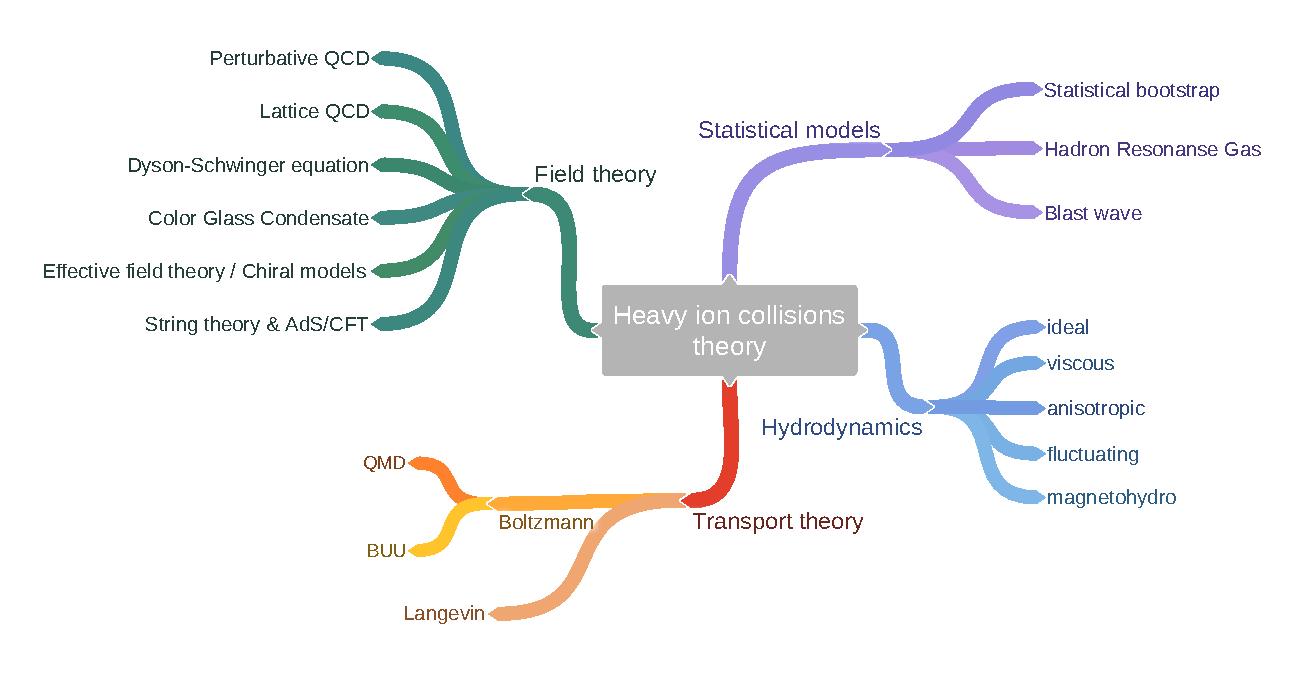
\includegraphics[width = \textwidth]{illustrations/intro_illustrations/Heavy_ion_collisionstheory.pdf}
  \caption{Theoretical approaches to heavy ion collisions.}
  \label{fig:HIC_th_mindmap}
\end{figure}


The theory of heavy ion collisions is rather versatile: the approaches range
from completely microscopic and static lattice QCD to macroscopic relativistic
hydrodynamics. The theoretical approaches may be divided into four branches as
shown in Fig. \ref{fig:HIC_th_mindmap}: field-theoretical, transport,
hydrodynamical and statistical. This thesis is devoted mainly to transport and
hydrodynamical approaches, as well as their fusion called hybrid approaches. That
is why the discussion about them is more extensive.  The other approaches are just
briefly listed here supplied with short descriptions, underlining their connections
to hydrodynamics and transport.

\subsection{Quantum chromodynamics} \label{sec:QCD}


The modern microscopic theory describing interactions of quarks and gluons is
quantum chromodynamics (QCD). Its Lagrangian is composed of interacting quark
fields $\ket{\Psi}$, which carry flavor, color and spin indices (therefore $6
\times 3 \times 4$ components) and gluon fields $A$ with Lorentz indices and a
color index taking 8 possible values corresponding to the number of
$\SUgroup{3}$ generators (see appendix \ref{sec:SU3}):

\begin{align} \label{eq:qcd_lagrangian}
  \mathcal{L} = - \sum_f \overline{\Psi}_f \sqbracs{ \gamma^{\mu} \partial_{\mu} -
                   \frac{i}{2} g \gamma^{\mu} A_{\mu}^a \lambda_a - m_f
                 } \Psi_f - \frac{1}{4} G_{\mu\nu}^a G^{\mu\nu}_a  \\
  G^{\mu\nu}_a = \partial_{\mu} A^{\nu}_a - \partial_{\nu} A^{\mu}_a +
                  f^{abc} A^{\mu}_b A^{\nu}_c
\end{align}

Here $\lambda_a$ are the Gell-Mann matrices introduced in appendix \ref{sec:SU3},
$f^{abc}$ are $\SUgroup{3}$ structure constants,
$\sqbracs{\frac{\lambda_a}{2},\frac{\lambda_b}{2}} = f^{abc}\frac{\lambda_c}{2}$.
Parameters of the QCD Lagrangian are the quark masses $m_f$ and the interaction constant $g$.
In principle, this Lagrangian contains the full description of strong interactions,
but the equations arising after quantizing it are notoriously hard to solve.
%Using QCD Lagrangian after quantization one can compute radiative corrections
%to scattering amplitudes. In QCD, as in many other quantum field theories, they
%turn out to be infinite.  To avoid infinities, the integrals are regularized by imposing a
%cut-off or other method, e.g. using $\overline{\mathrm{MS}}$ scheme. This
%procedure involves an energy cut-off scale $\mu^2$. Then counter-terms are added to
%the Lagrangian to compensate the infinity, which was cut away
%\cite{Kazakov:2008tr}. This method is called renormalization. The theory is
%called "renormalizable" if these compensating counter-terms only change the
%parameters of Lagrangian.

\begin{figure}
  \centering
  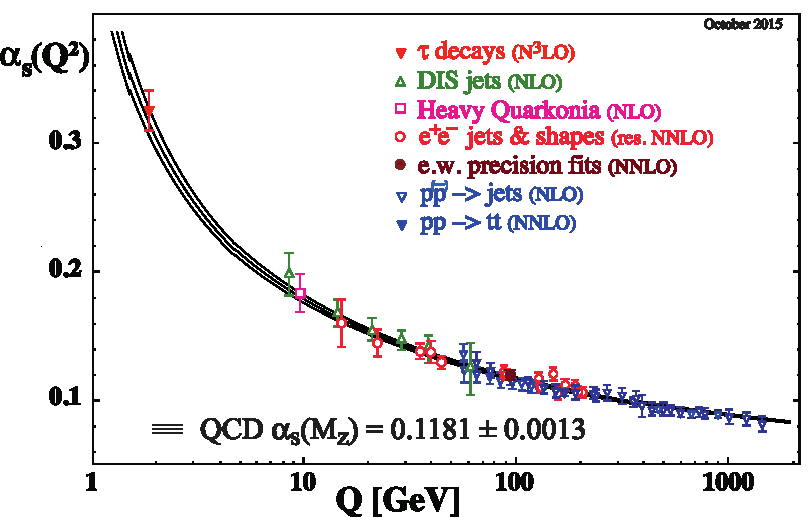
\includegraphics[width = 0.6\textwidth]{illustrations/intro_illustrations/asymptotic_freedom.pdf}
  \caption{Dependence of strong coupling constant on the energy scale. The
           decrease of coupling with energy scale is called asymptotic freedom.}
  \label{fig:asymptotic_freedom}
\end{figure}

QCD is a renormalizable theory \cite{Kazakov:2008tr} and after
renormalization the dependence of parameters $g(\mu^2)$ and $m_f(\mu^2)$ emerges,
where $\mu$ is the energy scale.
The first calculation of $g(\mu^2)$ was performed in 1973 by David Gross, Frank
Wilczek and David Politzer. They received the Nobel Prize in 2004 for this calculation.
Their main result can be expressed as follows \cite{Gross:1998jx} in terms of $\alpha_s =
\frac{g^2}{4\pi}$:

\begin{align} \label{eq:qcd_running_coupling}
  \frac{d\alpha_s}{d \, \lnOf{\mu}} = \frac{\alpha_s^2}{\pi} \beta_1 +
                                           \parenths{\frac{\alpha_s^2}{\pi}}^2 \beta_2 + \dots \\
  \beta_1 = - \sqbracs{\frac{11}{6}N_c - \frac{2}{3} n_f}
\end{align}

Here $N_c = 3$ is the number of colors and $n_f = 6$ is the number of flavors. One
 can see that $\beta_1$ is negative, so the coupling decreases with the energy scale $\mu$.
This means that the interaction between quarks at high energies or equivalently
 at small distances vanishes. This conclusion was confirmed by many
scattering experiments, see Figure \ref{fig:asymptotic_freedom}. 
The effect itself is called asymptotic freedom. Although quarks are always confined,
asymptotic freedom provides the chance to observe quasi-free quarks.
This possibility was an important motivation for heavy ion collisions,
until it has been realized that even at the highest LHC energies the quark-gluon plasma
is still strongly coupled. Indeed, the scale $\mu$ in Eq. (\ref{eq:qcd_running_coupling})
is set not by the very high collision energy $\sqrt{s}$, but by the temperature
of the formed medium, which is below 1 GeV.

Besides providing the motivation for heavy ion studies, perturbative QCD is
used to compute jet production cross-sections and jet quenching at high $p_T$
in the quark-gluon plasma. Also multiple perturbative calculations were
performed for finite-temperature QCD to determine quark-quark potentials in the
quark-gluon plasma \cite{Gross:1980br}. Perturbative calculations are
useful at high energies, where the strong-coupling constant is small according
to the Eq. (\ref{eq:qcd_running_coupling}). However, when $\mu$ decreases
the QCD coupling diverges at the scale of $\Lambda_{QCD} \sim $ 300 MeV \cite{Bruno:2017lta}.
One of the consequences is that perturbative QCD cannot deal with hadrons. This
gap is bridged by lattice QCD, described further and by other field-theoretical
approaches described in section \ref{sec:other_field_theories}.

Lattice QCD is a non-perturbative approach to QCD based on path integrals in a
discretized space-time. There are many ways to discretize the QCD action, but all
of them should converge to the same results in the continuum limit $a \to 0$
and $N_{\tau} \to \infty$, where $a$ is lattice spacing and $N_{\tau}$ is number
of points in Euclidean time. Within lattice QCD the lower lying part of the hadronic
spectrum can be computed, but most importantly for heavy ion physics it provides the
equation of state of strongly-interacting matter at zero chemical potential.
Due to Taylor expansion in $\frac{\mu}{T}$ at $\mu = 0$ the lattice QCD
equation of state is available in the region $\frac{\mu_b}{T} \le 2$
\cite{Borsanyi:2013bia,Bazavov:2014pvz,Bazavov:2017dus}. This
equation of state is widely used in hydrodynamical approaches. Lattice QCD
calculations are extremely computationally demanding, so many simplifying
assumptions are often made: large quark masses, massless quarks or small
$N_{\tau}$. Calculations with physical masses in (2+1)-flavor QCD (meaning that two
light quarks with equal masses and a strange quark are considered) and with
continuum extrapolation are only recently feasible \cite{Borsanyi:2014rza}.


\subsection{Other field-theoretical approaches} \label{sec:other_field_theories}

Field-theoretical approaches are mostly based on the QCD Lagrangian (see Eq.
\ref{eq:qcd_lagrangian}). As mentioned before, perturbative QCD cannot deal
with low-energy phenomena. This gap is partially bridged by
non-perturbative Dyson-Schwinger equations involving dressed quark and gluon
propagators \cite{Bashir:2012fs}.  They are rigorous, based on QCD and able to
capture physics at all energy scales, but unfortunately this is an infinite
system of equations that requires truncation. Other approaches covering
low-energy physics are effective field theories, where the degrees of freedom
are hadrons, not quarks or gluons \cite{Manohar:1996cq}. Such approaches are
usually based on the concept of chiral symmetry. These approaches are able to
predict hadronic cross-sections, decay widths and branching ratios, which then
can be inserted as an input to transport models. The disadvantage of effective
field theories is that they are non-renormalizable and therefore their
precision is limited and the applicability range is restricted
to low collision energies. Additionally, every hadron species needs to be inserted
should by inserted to the effective theory Lagrangian explicitly,
making realistic and detailed calculation extremely elaborate.

While chiral effective theories are applied at low energies, at high energies
the effective theory called Color Glass Condensate (CGC)
\cite{Gelis:2010nm,Iancu:2003xm} is useful. Proton-proton or nucleus-nucleus
collisions involve two energy scales: the large (''hard'') scale of the
parton-parton collision energy and the small (''soft'') scale of
inter-parton interactions within the nucleons. The computation of the reaction
cross-sections is possible within perturbative QCD for the 
parton-parton scattering. The soft part is neither accessible by perturbative
QCD nor by lattice QCD, so it is encapsulated into the parton distribution
functions (PDF) \cite{Pumplin:2002vw,Gluck:1994uf} measured mainly by
experiments at HERA $e^-p$ collider in Hamburg. PDFs depend on two parameters -
the momentum transfer $Q^2$ and the variable $x$ which
corresponds, at lowest order in perturbation theory, to the longitudinal
momentum fraction carried by a parton in the hadron. For small $x$ gluon PDFs
dominate in the nucleons, so one can say that at small $x$ nucleons consist
of a large number of gluons.

CGC is based on the concept of saturation, which can be explained as follows.
Schematically one can write a factorization theorem for the hadronic cross-sections:

\begin{equation}
  \sigma_{pp} = \int_0^1 dx_1 dx_2 \, PDF(x_1,Q^2) PDF(x_2,Q^2)
  \sigma_{partonic}\left(x_1,x_2,Q^2,\alpha_s(\mu^2),\frac{Q^2}{\mu^2}\right)
\end{equation}

The total cross-section should be limited. This follows from unitarity
\cite{Froissart:1961ux} and poses a restriction on the parton distribution function at
low $x$: PDFs should grow not faster than $\mathcal{O}\parenths{\frac{\log 1/x}{x}}$
for small enough $x$, $x < x_s(Q^2)$ - a phenomenon called saturation. Instead of
$x < x_s(Q^2)$ condition for fixed $Q^2$ one can also introduce $Q^2 > Q_s^2(x)$
condition for a fixed $x$. These considerations allow the CGC approach to separate
small $x$ and large $x$ physics. Within the CGC the nucleons are approximated as a combination of
classical gluon fields at small $x$ and valence quarks at large $x$ as sources of
these fields. The CGC picture is applicable for the very initial state of heavy ion collisions,
but at time of order $Q_s^{-1}$ the gluon medium becomes dilute and the 
basic assumption of saturation is no longer reached.  A suggested solution is to couple CGC
initialization to hydrodynamics \cite{Hirano:2005xf} or transport approaches
\cite{Kurkela:2015qoa}.

Another set of approaches to the strongly coupled regime inaccessible by
perturbative QCD is exploiting dualities between strongly coupled quantum
field theories and weakly-coupled gravitational theories, such as the  famous
AdS/CFT duality \cite{Maldacena:1997re}. This kind of approach was used to compute
the shear viscosity to entropy density ratio $\frac{\eta}{s}$ in a strongly-coupled
conformal field theory and find the well-known low value of $\frac{\eta}{s} =
\frac{1}{4\pi}$ \cite{Kovtun:2004de}.  The gauge-gravity duality has also been
applied to study the approach of fireball in heavy ion collisions to equilibrium
\cite{Chesler:2015lsa}.  Moreover, the whole heavy ion collision process at
high energies can be considered as a dual of two gravitational shock waves
colliding \cite{Arefeva:2016lcz}. Although very powerful, duality approaches
for heavy ion collisions can currently serve only for qualitative insights,
since no dual theory of QCD has yet been found.

\subsection{Statistical approaches}

Statistical approaches avoid describing the complex evolution of the fireball
in heavy ion collisions. Instead it is assumed that at chemical freeze-out all
the hadrons are in thermal and chemical equilibrium at the same temperature
$T$.  This allows to describe the fireball at freeze-out as an ideal gas of
hadrons and hadronic resonances. The inclusion of resonances as degrees of
freedom encapsulates hadron-hadron interactions according to the Bernstein-Dashen-Ma
theorem \cite{Dashen:1969ep}. The latter assumes that hadron interactions
proceed via narrow resonances, which is not always true: for example see Fig.
\ref{fig:xs} for $pp$ cross-section, which has no resonant structures.
Under the mentioned assumptions in the grand-canonical ensemble for an
ideal Boltzmann gas one obtains

\begin{equation}
  N_{i} = \frac{g_i V e^{\mu_i/T}}{2\pi^2} T^3 \parenths{\frac{m_i}{T}}^2 K_2\parenths{\frac{m_i}{T}} \,,
\end{equation}

where $N_i$ is the multiplicity of the hadron species $i$, $g_i$ is its degeneracy
and $m_i$ is its mass. This equation has to be supplied with conservation laws to
fix chemical potentials, resonance decays have to be taken into account for
comparison with experimental data and various corrections are possible - see
\cite{Andronic:2005yp,Oliinychenko:2012hj} for details. The overall model is
called Hadron Resonance Gas (HRG) model.  Although the HRG model is very simple and
its assumptions are rather naive, it describes hadron multiplicities in heavy
ion collisions remarkably well from AGS to LHC energies with three parameters:
the temperature $T$, the baryon chemical potential $\mu_b$ and the volume $V$
\cite{Becattini:2000jw,Andronic:2003zv,Andronic:2005yp,Cleymans:2005xv,Andronic:2008gu,Andronic:2011yq}.
Hadron Resonance Gas was also applied in the canonical ensemble with respect to strangeness conservation
\cite{Hagedorn:1984uy,Cleymans:1998yb,Begun:2006uu}. In the canonical ensemble
hadron multiplicities in $pp$ collisions \cite{Hamieh:2000tk}
and even $\epluseminus$ collisions \cite{Andronic:2008ev} can be described,
although for the latter the description quality is not as high.

The parameters $T(\sqrt{s})$, $\mu_b(\sqrt{s})$ and $V(\sqrt{s})$ extracted
from the fits to multiplicities at different collision energies $\sqrt{s}$
exhibit characteristic meaningful patterns.  Temperature of freeze-out $T$
increases with collision energy and saturates at around 160 MeV.
The chemical potential decreases with collision energy and goes to zero at LHC,
while the volume $V$ behaves exactly as the volume extracted from HBT radii - it
has a minimum at SPS energies. The saturation of the temperature may be explained
by the statistical bootstrap model by Hagedorn
\cite{Rafelski:2016hnq,Hagedorn:1965st}, which describes hadrons as ''bags''
being composites of one another. The bootstrap model yields an exponential hadron
spectrum and it originally predicted a limiting temperature $T_H \simeq $
150-170 MeV, above which hadrons cannot exist. This limiting
temperature was later reinterpreted as a transition temperature from hadrons to
quarks \cite{Cabibbo:1975ig}. It is believed that the value at which the freeze-out
temperature saturates is the Hagedorn temperature $T_H$ \cite{Andronic:2005yp}.

The Hadron Resonance Gas model only allows to describe hadron multiplicities. To
access momentum and rapidity spectra HRG was extended by including the overall
motion of the hadron gas. A freeze-out at some predefined hypersurface is
performed according to the Cooper-Frye formula \cite{Cooper:1974mv}. Such
models are called blast-wave models. They have the freedom to select the
freeze-out hypersurface, so there are several
modifications~\cite{Siemens:1978pb,Schnedermann:1993ws,Chojnacki:2011hb}.
Blast-wave models allow to describe transverse hadronic spectra using a common
radial expansion velocity $\beta$ common for all hadron species as an additional parameter.
Generally, blast-wave models are not able to produce higher-order flows: $v_2$,
$v_3$, etc. The description of anisotropic flow requires more involved dynamical approaches.

The temperatures $T_{kin}$ obtained from the blast wave fits to spectra are
typically lower than the temperatures $T_{chem}$ from HRG fit of multiplicities.
This is because inelastic reactions that change chemical content cease earlier than
pseudoelastic and elastic reactions that can only modify spectra. In other words,
chemical freeze-out happens earlier, when the temperature of the medium is higher.
The kinetic freeze-out, after which the spectra are not modified, occurs later.

\subsection{Hydrodynamic approaches} \label{sec:hydro_appr}

In contrast to statistical models, hydrodynamical approaches describe the
evolution of the fireball starting from thermalization until the
freeze-out.  Two necessary applicability conditions of hydrodynamics are
that every part of the system is in the vicinity of local thermal
equilibrium and the mean free path is much smaller than the system size,

\begin{equation} \label{eq:hydro_applicability}
  l_{mfp} \ll L \,.
\end{equation}

Typical expansion velocities in heavy ion collisions are comparable to the
speed of light, so the hydrodynamical theory must be relativistic.
Relativistic hydrodynamics was initiated in 1953 by the works of Landau for
multiparticle production in high-energy collisions of proton-proton,
proton-nucleus or nucleus-nucleus collisions\cite{Landau:1953gs,Belenkij:1956cd}. The
Landau model assumed high collision energy, so that two colliding nuclei are
represented as flat disks due to Lorentz contraction.  After colliding these
two disks stop completely and the resulting flat disk expands
longitudinally.  The model predicts a Gaussian rapidity spectrum, which was
indeed observed at AGS and SPS for the net charge.  At higher energies nuclei
do not seem to stop as rapidly as the Landau model assumes, but rather pass through
each other.  This is represented by the flat region of $dN/dy$ at midrapidity.
Such a situation is described well by the Bjorken hydrodynamical model
\cite{Bjorken:1982qr}, which assumes longitudinal boost invariance. The Bjorken
model allows to make a simple estimate of the energy density achieved in the
collision, which is used to judge by a comparison to the critical energy density
of $1$ GeV/fm$^3$, if the quark-gluon plasma was produced.

Modern approaches (recent overview \cite{deSouza:2015ena}) go far beyond these
approximations. However, the main equations of hydrodynamics, which are nothing
else but conservation of energy, momentum and charges, are written in the same
form as in the seminal papers of Landau \cite{Landau:1953gs,Belenkij:1956cd}:

\begin{align}
\partial_{\mu}\Tmn = 0 \\
\partial_{\mu}\jmu = 0 \,,
\end{align}

where $\Tmn$ is the energy-momentum tensor of the fluid and $\jmu$ is a
4-current of conserved charges. What has changed is

\begin{itemize}
  \item the dimensionality of the problem
  \item the equation of state (EoS)
  \item the initial conditions and event-by-event simulations
  \item the freeze-out conditions
  \item viscous corrections
\end{itemize}

In the following these aspects are described in more detail in this order.
Transverse expansion is included in (2+1)D and (3+1)D simulation. This is
important to describe transverse flow, in particular the dependence of
 $v_2(p_T)$, where $v_2$ is the second Fourier harmonics of the azimuthal angle distribution
 $\frac{dN}{d\varphi}$. Unlike the Landau or Bjorken models, these
 partial differential equations are not analytically solvable and have to
 be solved numerically.

The equation of state closes the system of hydrodynamic evolution equations,
connecting pressure with energy density and conserved charge densities:

\begin{equation}
 p = p (\epsilon, n)
\end{equation}

All the properties of the fluid are encoded in the EoS.  It is a big advantage
of the hydrodynamics that the EoS can be explicitly varied.  In this way one
can study the implications of the conjectured quark-gluon plasma to hadron gas
phase transition on the experimental observables \cite{Pang:2016vdc}. At low
$\mu_b$ the EoS is constrained by lattice QCD, but at higher $\mu_b$ it can
only be conjectured using phenomenological models.

The initial condition for hydrodynamics is the energy density $\epsilon(x,y,z)$ and
the baryon density $n_b(x,y,z)$ at a fixed time $t$ or at a fixed proper time
$\tau = \sqrt{t^2 - z^2}$, where the $z$-axis is along the beam direction.  Initial
conditions play an important role as they provide spatial anisotropies, which then
develop into momentum anisotropies $v_n$ measured in experiment. In earlier studies
initial conditions were smooth and based on the overlap geometry of the colliding
nuclei, see \cite{Huovinen:2006jp} for a review. In recent works they are
typically lumpy and generated by microscopic transport models
\cite{Petersen:2008dd,Karpenko:2015xea,Pang:2012he}, Color Glass Condensate
approach \cite{Lappi:2006xc,Schenke:2012wb}, IP-Glasma \cite{Gale:2012rq},
Monte Carlo versions of the Kharzeev-Levin-Nardi (MC-KLN)
\cite{Albacete:2011fw,Drescher:2006ca} or the Glauber model (MC-Glauber)
\cite{Miller:2007ri,Broniowski:2007nz,Loizides:2014vua}. Some approaches were
developed to classify this zoo \cite{ColemanSmith:2012ka}, but the true
initial condition is still to be found.

Because of the initial state fluctuations from collision to collision,
event-by-event calculations have to be performed. Instead of smooth averaged initial condition and
one hydrodynamic evolution one performs many simulations with different
initial conditions and then averages results.  These approaches are not
equivalent, since hydrodynamical equations are nonlinear.  Event-by-event
simulations are necessary to reproduce the higher flow harmonics, from $v_3$ up to
$v_6$ \cite{Gardim:2011xv,Auvinen:2013sba,Noronha-Hostler:2016opk}.

The earlier hydrodynamical simulations were stopped at a fixed time or proper
time, a so-called isochronous freeze-out. In modern simulations the freeze-out is
typically performed at a fixed temperature, energy density or Knudsen number.
Freeze-out is discussed in more detail in chapter \ref{chap:cooper_frye}.

In ideal hydrodynamics the energy momentum tensor in the rest frame of the fluid
element is written as

\begin{equation} \label{eq:id_fl_tmn_rest_frame}
    \Tmn_{\mathrm{ideal}} = \left(
    \begin{array}{cccc}
           \epsilon & 0 & 0 & 0 \\
           0        & p & 0 & 0 \\
           0        & 0 & p & 0 \\
           0        & 0 & 0 & p
    \end{array} \right) \,,
\end{equation}

where $\epsilon$ is local energy density and $p$ is pressure. Suppose that
the local fluid velocity is $\vec{\beta}$. Then the four-velocity takes the following form

\begin{equation}
  u^{\mu} = (\gamma, \gamma \vec{\beta}) \,,
\end{equation}

where $\gamma = \parenths{1 - \beta^2}^{-1/2}$. To boost the energy-momentum
tensor to the laboratory frame one multiplies it by Lorentz-matrices:

\begin{equation}
  \Tmn = \Lambda^{\mu}_{\alpha} \Lambda^{\nu}_{\beta} T^{\alpha \beta}
\end{equation}

\begin{equation} \label{eq:lorentz_boost_matr}
  \Lambda^{\mu}_{\nu} = \left(
    \begin{array}{cc}
           \gamma              & -\gamma \vec{\beta} \\
           -\gamma \vec{\beta} & \delta_{ij} + (\gamma - 1) \frac{\vec{\beta_i} \vec{\beta_j}}{\beta^2}
    \end{array} \right) = \left(
    \begin{array}{cc}
           u^0  &   -u^i  \\
           -u^i &  \delta^{ij} + (1+u^0)^{-1} u^i u^j
    \end{array} \right)
\end{equation}

Therefore, in the laboratory frame

\begin{equation} \label{eq:tmn_id_fluid}
  \Tmn_{\mathrm{ideal}} = \epsilon u^{\mu} u^{\nu} - p (g^{\mu\nu} - u^{\mu}u^{\nu}) \,,
\end{equation}

where $g^{\mu\nu} = \mathrm{diag}(1, -1, -1, -1)$. In ideal hydrodynamics the
four-current is a vector $(n,0,0,0)$, where $n$ is the density, boosted to the
laboratory frame:

\begin{equation} \label{eq:jmu_id_fluid}
  \jmu = n u^{\mu}
\end{equation}

Ideal hydrodynamics requires strict local thermodynamic equilibrium and
neglects possible dissipative effects. Small departures from local
equilibrium and dissipation are taken into account by  viscous
hydrodynamics. The equations of dissipative relativistic fluid dynamics
were first formulated by Eckart \cite{Eckart:1940te} and then by Landau and
Lifshitz \cite{LL_hydro}. Both were relativistic generalizations of
Navier-Stokes theory and are often referred to as first order theories. It
turned out that these generalizations are acausal, i.e. the speed of sound can
exceed the speed of light.  This was remedied in the Israel-Stewart second
order hydrodynamics \cite{Israel:1979wp}.  Recently a systematic expansion in
Knudsen number has been developed \cite{Denicol:2012cn}, which improves on the
14-moment approximation of Israel and Stewart.

Viscous hydrodynamics is applied with great success to simulate heavy ion
collisions
\cite{Teaney:2003kp,Romatschke:2007mq,Luzum:2008cw,Schenke:2010rr,Song:2007fn}.
It allows to describe anisotropic flow from $v_2$ to $v_6$ up to $p_T = $ 2.5 GeV
at RHIC and LHC, extract shear viscosity $\eta/s$ and bulk viscosity $\zeta/s$
and even some attempts to obtain the temperature dependence of $\eta/s$ from
experimental data are being made
\cite{Molnar:2014zha,Niemi:2015bpj,Karpenko:2015xea}.

A recent development is anisotropic hydrodynamics
\cite{Strickland:2014pga,Bazow:2013ifa}. Unlike the usual viscous
hydrodynamics, which is an expansion near thermal equilibrium, anisotropic
hydrodynamics expands around a non-equilibrium anisotropic state. This makes it
applicable for the early stages of heavy ion collisions, where the momentum anisotropy
is very large and conventional hydrodynamics cannot be applied.

\subsection{Transport approaches} \label{sec:transport}

The most general microscopic approaches to heavy ion collisions that consider
non-equilibrium evolution are approaches based on relativistic transport theory
\cite{de_Groot}.  Transport theory is formulated in terms of the
one-particle distribution function $\mathit{f}(t,\vec{r},\vec{p})$, which is
nothing else but the density in phase space. Assuming that the number of
particles in a given region of phase space can change only via collisions and
decays and neglecting all other sources of correlations one can write

\begin{equation} \label{eq:boltzmann}
  \frac{d\mathit{f}}{dt} = \frac{\partial\mathit{f}}{\partial t} +
                           \frac{\partial\mathit{f}}{\partial \vec{r}} \frac{p}{E} +
                           \frac{\partial\mathit{f}}{\partial \vec{p}} \vec{\nabla}U  = I_{coll} \,,
\end{equation}

where $I_{coll}$ is an expression called collision integral. This is the
non-relativistic classical Boltzmann equation, but it is nevertheless relevant for
quantum systems. It can be derived from the quantum BBGKY-hierarchy of
equations for the $N$-particle density matrix, truncating it at the two-particle
level and performing a Wigner transformation. This truncation assumes that the density
is not too high:

\begin{equation} \label{eq:transport_appl}
  \lambda_{\mathrm{Compton}} \ll l_{mfp} \,,
\end{equation}

where $\lambda_{\mathrm{Compton}} = \frac{hc}{M}$ is the Compton wavelength and
$l_{mfp} \simeq (\rho \sigma)^{-1}$ is the mean free path. This defines
the limit of applicability for the Boltzmann equation, which can however be overcome by
introducing different degrees of freedom. Another assumption made during the
truncation is the so-called hypothesis of molecular chaos:

\begin{equation} \label{eq:molecular_chaos}
  \mathit{f}_2(p_1,x_1;p_2,x_2) = \mathit{f}(p_1,x_1) \mathit{f}(p_2,x_2) \,,
\end{equation}

which implies the neglection of all phase space-correlations between particles.
The collision integral is written for the classical case as

\begin{equation}
  I_{coll} = \int \frac{d^3p_2}{E_2} \frac{d^3p'_1}{E_1} \frac{d^3p'_2}{E'_2}
          \times W(p,p_2 \to p'_1, p'_2) \times (f'_1 f'_2 - f f_2) \,.
\end{equation}

In the quantum case, the Boltzmann equation was first formulated by Uehling and Uhlenbeck and
therefore the equation is called BUU (Boltzmann-Uehling-Uhlenbeck):

\begin{equation} \label{eq:buu_icoll}
  I_{coll} =  \int \frac{d^3p_2}{E_2} \frac{d^3p'_1}{E_1} \frac{d^3p'_2}{E'_2}
          \times W(p,p_2 \to p'_1, p'_2) \times (f'_1 f'_2(1 + af)(1 + af_2) - f f_2 (1 + af'_1) (1 + af'_2)) \,.
\end{equation}

Here $a = 1$ for bosons and $a = -1$ for fermions. One can see that the quantum BUU
equation differs from the classical Boltzmann only by factors that account for
quantum statistics in the collision term.

The physical meaning of Boltzmann or BUU equations is very simple: for a given time interval $dt$
the number of particles in a phase-space cell has changed (left part) as much as
the number of particles that entered it from other cells via collisions or decays
(right part, gain term) minus the number of particles that escaped to other cells
via collisions or decays (right part, loss term). The Boltzmann equation can be
written in a manifestly covariant notation:

\begin{equation} \label{eq:Boltz}
  p^{\mu}\frac{\partial\mathit{f}}{\partial x^{\mu}} +
  m \frac{\partial K^{\mu}\mathit{f}}{\partial p^{\mu}} = I_{coll} \,,
\end{equation}

where $K^{\mu}$ is Minkowski-four-force vector. The Boltzmann equation as written above
is just for one sort of particles experiencing $2\to 2$ elastic collisions. In heavy ion
collisions one encounters hundreds of different hadrons, that can also collide inelastically,
decay and form resonances. For this case
Boltzmann equation turns into a coupled system of equations - as many equations
as hadron species. This system is generally solved via Monte-Carlo
simulations, where the particles propagate according to the equations of motion
obtained from the left hand side of Eq. \ref{eq:Boltz} and collide/decay
simulating the collision integral.

Depending on the degrees of freedom, there are pure hadronic transport codes,
used at low energies
\cite{Aichelin:1986wa,Ko:1989se,Pang:1992fg,Hartnack:1989sd,Cassing:1990dr},
approaches including hadrons and strings (e.g., RQMD \cite{Sorge:1989vt}, UrQMD
\cite{Bass:1998ca}, HSD \cite{Cassing:2000bj}, JAM \cite{Nara:1999dz}, GiBUU
\cite{Buss:2011mx}), only partons (e.g., \cite{Geiger:1991nj,Molnar:2004yh},
Zhang Parton Cascade \cite{Zhang:1997ej}, BAMPS \cite{Xu:2004mz}) or partons,
hadrons and string together, like PHSD \cite{Cassing:2008sv} or AMPT
\cite{Lin:2004en}.

Transport simulations are divided into two groups, usually called BUU
(Boltzmann-Uehling-Uhlenbeck) and QMD (Quantum Molecular Dynamics), which
differ in the treatment of potentials. BUU approaches aim at solving the one-body
BUU equations with mean-field potentials depending on the local density. The
hypothesis of molecular chaos implies that in BUU approaches all the
correlations between particles are destroyed. The QMD approach solves equations
of motion for particles with potentials depending on distances and momenta. The
QMD approach generates correlations between particles. In the case in which there are no
potentials, which is called the cascade mode, QMD and BUU approaches are
identical.

Transport approaches are extremely powerful tools to study heavy ion collisions,
because they do not require local equilibrium, simulate microscopic interactions
and allow to extract almost any experimentally observable quantity. However, they
also have some disadvantages:

\begin{itemize}
  \item Strictly speaking, transport approaches are only applicable, if the density
        is low enough, so that Eq. \ref{eq:transport_appl} is fulfilled.
  \item A lot of phenomenological input is required. Many resonance cross-sections
        and branching ratios are not known experimentally. Modeling microscopically
        the hadronization process is challenging. String formation and fragmentation
        can be modeled in many possible ways. All this creates considerable
        differences in the results even between conceptually similar approaches,
        see e.g. this comparison \cite{Xu:2016lue}.
\end{itemize}

\subsection{Hybrid approaches} \label{sec:hybrid_appr}

%\begin{figure}
%  \centering
%  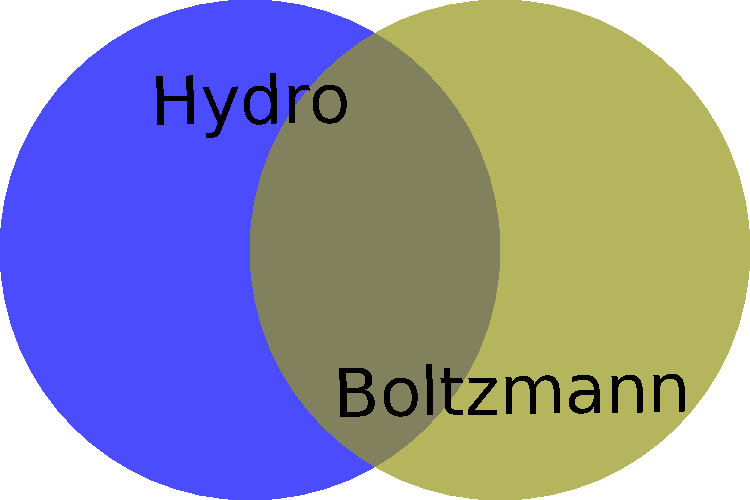
\includegraphics[width = 0.5\textwidth]{illustrations/intro_illustrations/hyd_boltz.pdf}
%  \caption{Schematic view on the regions of applicability of hydrodynamics
%           and Boltzmann equation.}
%  \label{fig:hyd_boltz}
%\end{figure}

As one can see from the applicability conditions for transport approaches (Eq.
\ref{eq:transport_appl}) and hydrodynamics (Eq. \ref{eq:hydro_applicability}),
transport tends to be applicable at lower densities and hydrodynamics at
higher densities. At the same time, the hydrodynamical equations can be derived
from the Boltzmann equation, therefore the regions of applicability of hydrodynamics
and transport overlap. 
This motivated the development of hybrid approaches, which use hydrodynamics at high
density and switch to transport at low density, hopefully in the region, where
both are applicable. Hybrid approaches are very successful in describing
experimental data at highest RHIC and LHC energies \cite{Bass:2000ib,Teaney:2001av,Hirano:2005xf,Nonaka:2006yn,Petersen:2008dd,Werner:2010aa,Song:2010mg,Karpenko:2012yf,Hirano:2012kj},
and for the RHIC beam energy scan \cite{Karpenko:2015xea,Auvinen:2016uuv}.

The advantages of hybrid approaches are:

\begin{itemize}
  \item Theoretical consistency: hydrodynamics and transport are supposed
        to be applied within their applicability ranges.
  \item The hadronic rescattering stage improves the description of experimental data
        compared to pure hydrodynamics, in particular it improves the description of
        elliptic flow $v_2$ of identified particles and
        $p_T$ spectra of protons and $\Lambda$ \cite{Petersen:2014yqa}.
  \item The equation of state can be studied explicitly.
  \item There are no uncertainties related to hadronization in the transport simulation.
        The complex hadronization process is encoded in the equation of state.
\end{itemize}

These advantages make hybrid approaches excellent simulations at intermediate
energies, relevant for RHIC beam energy scan, NICA, FAIR and JPARC. However, in
this thesis it is argued that some improvements of hybrid approaches are necessary
to perform consistent simulations at intermediate energies. These improvements
are connected to the interfaces between the hydrodynamics and transport.

Modern hybrid approaches assume:

\begin{enumerate}
  \item Fast thermalization and an ideal fluid form of energy-momentum tensor (Eq.
        \ref{eq:tmn_id_fluid}) at the initialization. At high energies these
        assumptions seem to be justified, however at intermediate energies they are
        not guaranteed. In chapter \ref{chap:local_equilibration} these
        assumptions are verified, testing the deviation of the energy-momentum
        tensor from ideal fluid form.
  \item At the initialization of hydrodynamics the whole space is assumed to be in thermal
        equilibrium. However, the borders of the fireball never really enter
        the equilibrated phase. This is cured in the core-corona approach
        \cite{Steinheimer:2011mp}, where the core with high energy density is treated
        by hydrodynamical equations and the low-density corona is propagated with
        transport. At high energies the corona is negligible, but at intermediate
        energies it becomes important. It has to be noted that in
        \cite{Steinheimer:2011mp}
        core and corona are decoupled: particles from the corona cannot feedback to
        the core.
        This is in line with the next assumption of hybrid approaches.
  \item It is assumed that transport is decoupled from hydrodynamics: particles from
        transport cannot cause any feedback to hydrodynamical equations. It turns
        out that this assumption becomes more and more challenging when one moves
        from higher energies to lower beam energies, as shown in chapter \ref{chap:cooper_frye}.
  \item The particlization hypersurface is chosen by hand. Typically, it is a hypersurface
        of constant energy density or temperature, where it is assumed that both
        hydrodynamics and transport are applicable. If this assumption is justified
        then at particlization hypersurface the amount of particles flying into
        the hydrodynamical region would be consistent with the hydrodynamical
        expectation. In chapter \ref{chap:cooper_frye} it is demonstrated that this
        conjecture is not fulfilled.
\end{enumerate}

I would like to underline that the listed assumptions are well-justified at
highest RHIC and LHC energies, where most of the hybrid approaches were applied,
but they are challenging at RHIC beam energy scan, NICA, FAIR and JPARC energies.

There is a number of approaches and ideas, which seek for relaxing these
assumptions. Anisotropic hydrodynamics \cite{Strickland:2014pga,Bazow:2013ifa}
is applicable for highly anisotropic initial states, which are out of equilibrium
in a particular way. As shown in chapter \ref{chap:local_equilibration}, the
departure from equilibrium in heavy ion collisions at intermediate energies is mainly
due to the pressure anisotropy. This means that anisotropic hydrodynamics is able to
relax the first assumption about fast thermalization.

The next assumptions could be relaxed in an approach, in which \emph{coupled}
hydrodynamical and transport equations are solved. Attempts to
write down the appropriate equations were already performed. Boundary conditions on
a sharp hypersurface separating two transport approaches with different
distribution functions were formulated in \cite{Bugaev:2002ch}. These conditions
are also suitable for the boundary between hydrodynamics and transport. However, it is not
enough to formulate the boundary conditions. One also has to supply the rules for
how particles thermalize or how they deposit energy entering the hydrodynamical
phase.

This was partially addressed in the hydrokinetic approach
\cite{Sinyukov:2002if,Akkelin:2008eh}, where particles decouple from
hydrodynamics continuously governed by rate equations. The decoupling
hypersurface is momentum dependent in such a way that particles do not
return to the hydrodynamical domain. There is also an approach of a transition
layer \cite{Csernai:2004pr,Molnar:2005gx}, where particle escape probabilities
are also governed by rate equations and particles returning to the hydrodynamical
domain are integrated out.

An approach, where coupled hydrodynamical and transport equations are solved and the
boundary is defined dynamically is not fully developed for the relativistic case.
However, the analogous non-relativistic problem often appears in practice and is solved
for many different scenarios. A possible example is the simulation
of fluid flow with complicated boundary conditions: at the boundary the fluid has
to be simulated kinetically and far from the boundary hydrodynamically.
This kind of non-relativistic problem is successfully solved using
the domain decomposition methods, see for example \cite{Tiwari:2009} and references
therein. Similar ideas are also used in plasma simulations, see
e.g.~\cite{Tuckmantel:2010}. An analogous approach for heavy ion collisions
would solve many of the problems that appear in the present hybrid models,
in particular the problem of negative Cooper-Frye contributions (section
\ref{sec:cf_explanation}).

In chapter \ref{chap:forced_therm} an alternative approach to the problem is
suggested. Hadronic transport is applied in the whole space, but in the region of
high energy density it is subjected to forced thermalization. This allows
to interpolate between transport and hydrodynamics. Unfortunately, varying
the equation of state in this approach is challenging, although possible in
principle. 	Hadrons inside the ''hydrodynamical'' high-density region
need then to be treated as fictitious particles like in the particle-in-cell
hydrodynamics \cite{Harlow:1976}.

